\section{スピンフリッパーの共鳴}

「共鳴」は物理の様々な場所で登場する。例えば音叉の共鳴。固有振動数の等しいふたつの音叉を用意し片方だけを鳴らす。するともう一方もひとりでに鳴り始める。固有振動数の異なる音叉ではこのような現象は起こらない。このように、系がある特定の振動数に対してのみ特異なふるまいをみせる現象を、物理では広く「共鳴」と呼ぶ。

%スピンフリッパーの共鳴とは、フリッパーで特定の周波数の振動磁場をかけたときにフリッパーを通り抜けたある速度の中性子のスピンが完全に反転してしまう現象をいう。本実験における干渉パターンの見えやすさを高めるために、スピンフリッパーの共鳴が必要となる。
ではスピンフリッパーの共鳴とはいったい何だろうか。何のために共鳴させるのだろう。その実現方法は。この章ではそれらについて説明した後、実際の実験で用いた装置と従った手順、得られたデータを示し、最後にデータの分析を行う。

\subsection{What?\ $\sim$スピンフリッパーの共鳴とは何か$\sim$} \label{Resonance_what}
共鳴条件()が満たされるとき、スピンフリッパーは共鳴しているという。その背後にどんな物理的意味が潜んでいるのだろうか。

\paragraph{舞台とあらすじ}
一様磁場中に理想化されたRFスピンフリッパーがひとつ置かれた状況を考える。系は3つの領域I,II,IIIからなり、全体に$z$方向一様磁場$B_z$が、領域IIに$x$方向振動磁場$2B_r \cos \omega_s t$がかけられている。
\begin{figure}[h]
\centering
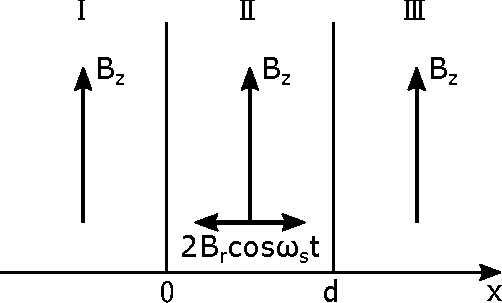
\includegraphics[height=3cm]{resonance/whatwhyhow/Resonance_what_setting.pdf}
\end{figure}

これから述べるように、スピン上向きの中性子が領域Iから速度$v$で入射し領域IIを通って領域IIIに抜けるとき、領域IIIにおけるスピン上向き中性子の存在確率は
\begin{equation}
|\psi_{\mathrm{III}}^+|^2=\cos^2 \frac{\omega_A}{v}d+\left(\frac{\epsilon}{\omega_A}\right)^2\sin^2\frac{\omega_A}{v}d \label{Resonance_flip}
\end{equation}
となる。ここで$\epsilon=\omega_s/2-\omega_z,\omega_A=\sqrt{\epsilon^2+\omega_r^2}$であり、$\omega_z=|\mu_n|B_z,\omega_r=|\mu_n|B_r$、$\mu_n$は中性子の磁気モーメント、$d$は領域IIの幅である。いま
\begin{equation}
\epsilon=\frac{\omega_s}{2}-\omega_z=0 \label{Resonance_resonance}
\end{equation}
がなりたてば、$\omega_rd/v=\pi/2$を満たす速度の中性子に対して、領域IIIにおけるスピン上向き粒子の存在確率が0、すなわちスピン反転率が1になることがわかる。逆に$\epsilon \neq 0$のときはどのような速度の中性子に対しても反転率は1となり得ない。このように、式(\ref{Resonance_resonance})を満たす周波数の振動磁場をかけたときに限りスピンフリッパーを通り抜けた中性子のスピンが完全に反転し得る。これをスピンフリッパーの共鳴と呼び、式(\ref{Resonance_resonance})を共鳴条件と呼ぶ。

\renewcommand{\arraystretch}{1.5}

%\begin{center}(中略)\end{center}


%\begin{comment}
\paragraph{入射波}
スピンの量子化軸を$z$軸に選ぶと、領域IにおけるShr$\ddot{\mathrm{o}}$dinger方程式は%なぜか\''{o}が使えない
\begin{equation}
i\frac{\del \psi_\mathrm{I}}{\del t}= \Biggl[-\frac{1}{2m} \frac{\del^2}{\del x^2} \underbrace{-\mu_nB_z}_{+|\mu_n|Bz =\omega_z} \sigma_z\Biggr] \psi_\mathrm{I}
\end{equation}
入射中性子のスピンは上向きとしたので、そのエネルギーを$\omega_0$とすると、領域Iにおける波動関数の入射成分はスピン上下の2成分表示で
\begin{equation}
\psi_\mathrm{I}^{\mathrm{in}}=\begin{pmatrix} 1\\0 \end{pmatrix} \e^{i k_0^+ x -i\omega_0 t}
\end{equation}
と書ける。ここで$k_0^+=\sqrt{2m(\omega_0 -\omega_z)}$。
\renewcommand{\arraystretch}{1}

\paragraph{領域II}
領域IIにおける磁場を
\begin{equation}
\bm{B}_{\mathrm{II}}=\hat{\bm{x}} (2B_r)\cos \omega_s t+\hat{\bm{z}} B_z
\end{equation}
と書く。ただし$\hat{\bm{x}},\hat{\bm{z}}$はそれぞれx,z軸正の向きの単位ベクトル。$|B_r| \ll |B_z|$のときには、\ref{pi2flipper_sec}章で述べた理由により振動磁場を次のような$xy$平面上の回転磁場に置き換えてよい:
\begin{equation}
\hat{\bm{x}} (2B_r)\cos \omega_s t \rightarrow \hat{\bm{x}} B_r \cos \omega_s t+\hat{\bm{y}} \sin \omega_s t
\end{equation}
したがって$|B_r| \ll |B_z|$のとき領域IIにおける磁場は
\begin{equation}
\bm{B}_{\mathrm{II}}\simeq \hat{\bm{x}} B_r\cos \omega_s t+\hat{\bm{y}} B_r \sin \omega_s t+\hat{\bm{z}} B_z
\end{equation}
となる。このとき領域IIにおけるShr$\ddot{\mathrm{o}}$dinger方程式は
\begin{align}
i\frac{\del \psi_{\mathrm{II}}}{\del t} &=\left[-\frac{1}{2m} \frac{\del^2}{\del x^2} -\bm{\mu}_n\cdot\bm{B}_\mathrm{II}\right] \psi_\mathrm{II}\notag \\
&=\left[-\frac{1}{2m} \frac{\del^2}{\del x^2} + |\mu_n| (\sigma_x B_r \cos\omega_s t+\sigma_y B_r\sin\omega_s t+\sigma_zB_z)\right] \psi_\mathrm{II} \notag \\
&=\left[-\frac{1}{2m} \frac{\del^2}{\del x^2} +\begin{pmatrix} \omega_z &\omega_r \e^{-i\omega_s t} \\\omega_r \e^{i\omega_s t} &-\omega_z \end{pmatrix}\right] \psi_\mathrm{II}
\end{align}
となる。まずハミルトニアンの時間依存性を除くために、$z$軸まわりの角速度$-\omega_s$の回転を表すユニタリ変換
\begin{equation}
U_T=\exp\left[+iS_z\omega_s t\right] =\exp\left[i\sigma_z\frac{\omega_s t}{2}\right]=\begin{pmatrix} \e^{i\omega_st/2} &0\\0&\e^{-i\omega_st/2}\end{pmatrix}
\end{equation}
を用いて
\begin{equation}
U_T \begin{pmatrix} \omega_z &\omega_r \e^{-i\omega_s t} \\\omega_r \e^{i\omega_s t} &-\omega_z \end{pmatrix} U_T^\dagger =\begin{pmatrix} \omega_z &\omega_r\\ \omega_r&-\omega_z \end{pmatrix}
\end{equation}
がなりたつことに注意すると、
\begin{equation}
i\frac{\del}{\del t}(U_T \psi_\mathrm{II}) =\left[-\frac{1}{2m} \frac{\del^2}{\del x^2} +\begin{pmatrix} -(\frac{\omega_s}{2}-\omega_z) &\omega_r\\ \omega_r &\frac{\omega_s}{2}-\omega_z \end{pmatrix}\right] (U_T \psi_\mathrm{II})
\end{equation}
を得る。さらにこのハミルトニアンを対角的にするために
\begin{equation}
\begin{pmatrix} -(\frac{\omega_s}{2}-\omega_z) &\omega_r\\ \omega_r &\frac{\omega_s}{2}-\omega_z \end{pmatrix}=\omega_A\begin{pmatrix} \cos \theta&\sin \theta\\ \sin \theta &-\cos \theta \end{pmatrix}
\end{equation}
と書く。ここで$\epsilon=\omega_s/2-\omega_z,\omega_A=\sqrt{\epsilon^2+\omega_r^2}$として
\begin{equation}
\cos \theta=\frac{-\epsilon}{\omega_A} , \quad \sin \theta=\frac{\omega_r}{\omega_A}
\end{equation}
である。$y$軸まわりの角度$-\theta$回転を表すユニタリ変換
\begin{equation}
U_D=\exp\left[+iS_y \theta\right] =\exp\left[i\sigma_y \frac{\theta}{2}\right] =\begin{pmatrix} \cos\frac{\theta}{2}& \sin\frac{\theta}{2}\\  -\sin\frac{\theta}{2}& \cos\frac{\theta}{2}\end{pmatrix}
\end{equation}
を用いて
\begin{equation}
U_D \begin{pmatrix} \cos \theta&\sin \theta\\ \sin \theta &-\cos \theta \end{pmatrix} U_D^\dagger =\begin{pmatrix} 1&0\\0&-1\end{pmatrix}
\end{equation}
がなりたつことに注意すると、
\begin{equation}
i\frac{\del}{\del t}(U_DU_T \psi_\mathrm{II}) =\left[-\frac{1}{2m} \frac{\del^2}{\del x^2} +\omega_A \sigma_Z \right] (U_DU_T \psi_\mathrm{II})
\end{equation}
を得る。

\renewcommand{\arraystretch}{1.5}
したがって、領域IIにおける中性子のエネルギーを$\omega_n$とすると、定数$A_n^\pm,B_n^\pm$を用いて
\begin{equation}
\psi_D \equiv U_D U_T \psi_\mathrm{II} =\begin{pmatrix} A_n^+ \e^{ik_n^+x}+B_n^+\e^{-ik_n^+x} \\ A_n^- \e^{ik_n^-x}+B_n^-\e^{-ik_n^-x} \end{pmatrix} \e^{-i\omega_n t}
\end{equation}
と書けるから、領域IIにおける波動関数は
\begin{align}
\psi_\mathrm{II}&=U_T^\dagger U_D^\dagger \psi_D \notag \\
&=\begin{pmatrix} \e^{-i\omega_st/2} &0\\0&\e^{+i\omega_st/2}\end{pmatrix} \begin{pmatrix} \cos\frac{\theta}{2}& -\sin\frac{\theta}{2}\\  \sin\frac{\theta}{2}& \cos\frac{\theta}{2}\end{pmatrix} \begin{pmatrix} A_n^+ \e^{ik_n^+x}+B_n^+\e^{-ik_n^+x} \\ A_n^- \e^{ik_n^-x}+B_n^-\e^{-ik_n^-x} \end{pmatrix} \e^{-i\omega_n t} \notag \\
&=\begin{pmatrix} \left(A_n^+ \cos \frac{\theta}{2} \e^{ik_n^+x}+ B_n^+ \cos \frac{\theta}{2} \e^{-ik_n^+x} - A_n^- \sin \frac{\theta}{2} \e^{ik_n^-x}- B_n^- \sin \frac{\theta}{2} \e^{-ik_n^-x}\right) \e^{-i(\omega_n+\omega_s/2)t} \\ \left(A_n^+ \sin \frac{\theta}{2} \e^{ik_n^+x}+ B_n^+ \sin \frac{\theta}{2} \e^{-ik_n^+x} + A_n^- \cos \frac{\theta}{2} \e^{ik_n^-x}+ B_n^- \cos \frac{\theta}{2} \e^{-ik_n^-x}\right) \e^{-i(\omega_n-\omega_s/2)t} \end{pmatrix} \label{Resonance_psi2}
\end{align}
と書ける。ここで$k_n^\pm=\sqrt{2m(\omega_n \mp \omega_A)}$。

\paragraph{領域IとIIの接続}
入射波$\psi_\mathrm{I}^\mathrm{in}$と$\psi_\mathrm{II}$が任意の時刻$t$で領域IとIIの境界($x=0$)において接続するためには
\begin{equation}
\omega_n=\omega_1 \equiv \omega_0 -\frac{\omega_s}{2}
\end{equation}
が必要である。そのとき
\begin{equation}
\psi_\mathrm{II}=\begin{pmatrix} \left(A_1^+ \cos \frac{\theta}{2} \e^{ik_1^+x}+ B_1^+ \cos \frac{\theta}{2} \e^{-ik_1^+x} - A_1^- \sin \frac{\theta}{2} \e^{ik_1^-x}- B_1^- \sin \frac{\theta}{2} \e^{-ik_1^-x}\right) \e^{-i\omega_0t} \\ \left(A_1^+ \sin \frac{\theta}{2} \e^{ik_1^+x}+ B_1^+ \sin \frac{\theta}{2} \e^{-ik_1^+x} + A_1^- \cos \frac{\theta}{2} \e^{ik_1^-x}+ B_1^- \cos \frac{\theta}{2} \e^{-ik_1^-x}\right) \e^{-i(\omega_0-\omega_s)t} \end{pmatrix}
\end{equation}
ここで$k_1^\pm=\sqrt{2m(\omega_0-\omega_s/2 \mp \omega_A)}$。

またこのことから、領域Iでの反射波を含めた全波動関数$\psi_\mathrm{I}$は
\begin{equation}
\psi_\mathrm{I} =I_0^+ \psi_\mathrm{I}^\mathrm{in} +\begin{pmatrix} R_0^+ \e^{-ik_0^+x}\e^{ -i\omega_0 t} \\ R_2^- \e^{-ik_2^-x}\e^{ -i (\omega_0-\omega_s)t} \end{pmatrix} =\begin{pmatrix} (I_0^+ \e^{ik_0^+x} +R_0^+\e^{-ik_0^+x} )\e^{-i\omega_0 t} \\ R_2^- \e^{-ik_2^-x}\e^{ -i (\omega_0-\omega_s)t} \end{pmatrix}
\end{equation}
と書ける。ここで$I_0^+,R_0^+,R_2^-$は定数であり、$k_0^+ =\sqrt{2m(\omega_0 -\omega_z)},k_2^- =\sqrt{2m(\omega_0 -\omega_s +\omega_z)}$である。

さて、ここで領域IとIIの接続を考えると、次の4つの式がなりたつ:
\begin{align}
\left\{\begin{array}{l}
A_1^+ \cos \frac{\theta}{2} +B_1^+\cos \frac{\theta}{2} -A_1^-\sin\frac{\theta}{2} -B_1^-\sin\frac{\theta}{2} = I_0^+ +R_0^+ \\
k_1^+(A_1^+ \cos \frac{\theta}{2} -B_1^+\cos \frac{\theta}{2} )-k_1^-(A_1^-\sin\frac{\theta}{2} -B_1^-\sin\frac{\theta}{2} )=k_0^+(I_0^--R_0^+)\\
A_1^+ \sin \frac{\theta}{2} +B_1^+\sin \frac{\theta}{2} +A_1^-\cos\frac{\theta}{2} +B_1^-\cos\frac{\theta}{2} = R_2^- \\
k_1^+(A_1^+ \sin \frac{\theta}{2} -B_1^+\sin \frac{\theta}{2}) +k_1^-(A_1^-\cos\frac{\theta}{2} -B_1^-\cos\frac{\theta}{2}) = -k_2^-R_2^-
\end{array} \right. \label{Resonance_setsuzoku}
\end{align}

\paragraph{近似}
いま中性子の入射エネルギー$\omega_0$は、$\omega_z$や$\omega_s,\omega_r$などと比べて十分大きいとする。このとき
\begin{align}
&k_0^+ =\sqrt{2m(\omega_0 -\omega_z)} \simeq k_0 -\frac{\omega_z}{v} \label{Resonance_k0+} \\
&k_1^{\pm} = \sqrt{2m(\omega_0-\omega_s/2 \mp \omega_A)} \simeq k_0 -\frac{\omega_s}{2v} \mp \frac{\omega_A}{v} \label{Resonance_k1+-} \\
&k_2^- =\sqrt{2m(\omega_0 -\omega_s +\omega_z)} \simeq k_0 -\frac{\omega_s}{v} +\frac{\omega_z}{v}\label{Resonance_k2-}
\end{align}
となる。ここで$k_0 \equiv \sqrt{2m\omega_0}$とした。さらに式(\ref{Resonance_setsuzoku})のように指数の肩以外に$k_n^\pm$が降りているときは
\begin{equation}
k_n^\pm \simeq k_0\label{Resonance_kn+-}
\end{equation}
と近似する。後で見るようにこれは反射波を無視することと同値である。

この近似の下で式(\ref{Resonance_setsuzoku})は次のように変形される:
\begin{align}
&\left\{\begin{array}{l}
A_1^+ \cos \frac{\theta}{2} +B_1^+\cos \frac{\theta}{2} -A_1^-\sin\frac{\theta}{2} -B_1^-\sin\frac{\theta}{2} = I_0^+ +R_0^+ \\
k_0(A_1^+ \cos \frac{\theta}{2} -B_1^+\cos \frac{\theta}{2} )-k_0(A_1^-\sin\frac{\theta}{2} -B_1^-\sin\frac{\theta}{2} )=k_0(I_0^--R_0^+)\\
A_1^+ \sin \frac{\theta}{2} +B_1^+\sin \frac{\theta}{2} +A_1^-\cos\frac{\theta}{2} +B_1^-\cos\frac{\theta}{2} = R_2^- \\
k_0(A_1^+ \sin \frac{\theta}{2} -B_1^+\sin \frac{\theta}{2}) +k_0(A_1^-\cos\frac{\theta}{2} -B_1^-\cos\frac{\theta}{2}) = -k_0R_2^-
\end{array} \right.  \notag \\
&\Rightarrow \left\{\begin{array}{l}
A_1^+ \cos \frac{\theta}{2} +B_1^+\cos \frac{\theta}{2} -A_1^-\sin\frac{\theta}{2} -B_1^-\sin\frac{\theta}{2} = I_0^+ +R_0^+ \\
A_1^+ \cos \frac{\theta}{2} -B_1^+\cos \frac{\theta}{2} -A_1^-\sin\frac{\theta}{2} -B_1^-\sin\frac{\theta}{2} =I_0^--R_0^+\\
A_1^+ \sin \frac{\theta}{2} +B_1^+\sin \frac{\theta}{2} +A_1^-\cos\frac{\theta}{2} +B_1^-\cos\frac{\theta}{2} = R_2^- \\
A_1^+ \sin \frac{\theta}{2} -B_1^+\sin \frac{\theta}{2} +A_1^-\cos\frac{\theta}{2} -B_1^-\cos\frac{\theta}{2} = -R_2^-
\end{array} \right.  \notag \\
&\Rightarrow \left\{\begin{array}{l}
A_1^+ \cos \frac{\theta}{2} -A_1^-\sin\frac{\theta}{2}= I_0^+ \\
B_1^+\cos \frac{\theta}{2} -B_1^-\sin\frac{\theta}{2} =R_0^+\\
A_1^+ \sin \frac{\theta}{2}+A_1^-\cos\frac{\theta}{2}= 0 \\
B_1^+\sin \frac{\theta}{2} -B_1^-\cos\frac{\theta}{2} = R_2^-
\end{array} \right.  \notag \\
&\Rightarrow \left\{\begin{array}{l}
A_1^+ = I_0^+\cos\frac{\theta}{2} \\
A_1^- =-I_0^+\sin\frac{\theta}{2} \\
B_1^+=R_0^+\cos\frac{\theta}{2}+R_2^-\sin\frac{\theta}{2} \\
B_1^-=R_2^-\cos\frac{\theta}{2}-R_0\sin\frac{\theta}{2}
\end{array} \right. \label{Resonance_1and2}
\end{align}

\paragraph{領域III}
領域IIIにおけるShr$\ddot{\mathrm{o}}$dinger方程式は領域Iと同じで
\begin{equation}
i\frac{\del \psi_\mathrm{III}}{\del t}= \left[-\frac{1}{2m} \frac{\del^2}{\del x^2} +\omega_z \sigma_z\right] \psi_\mathrm{III}
\end{equation}
である。$\psi_\mathrm{II}$と$\psi_\mathrm{III}$が任意の時刻$t$で領域IIとIIIの境界($x=d$)において接続するためには、式(\ref{Resonance_psi2})より、領域IIIにおける中性子のエネルギーがスピン上向きに対しては$\omega_0$、スピン下向きに対しては$\omega_0-\omega_s$であることが必要である。よって領域IIIにおける波動関数$\psi_\mathrm{III}$は定数$C_0^+,C_2^-$を用いて
\begin{equation}
\psi_\mathrm{III}=\begin{pmatrix} C_0^+ \e^{ik_0^+ x}\e^{-i\omega_0 t} \\ C_2^- \e^{ik_2^- x}\e^{-i(\omega_0-\omega_s) t} \end{pmatrix}
\end{equation}
と書ける。ここで$k_0^+=\sqrt{2m(\omega_0-\omega_z)},k_2^-=\sqrt{2m(\omega_0-\omega_s+\omega_z)}$。

\paragraph{領域IIとIIIの接続}
次に領域IIとIIIの接続を考える。前述の通り、波数の内、指数の肩に乗っているものについては式(\ref{Resonance_k0+}),(\ref{Resonance_k1+-}),(\ref{Resonance_k2-})のように、指数の肩から降りているものについては式(\ref{Resonance_kn+-})のように近似する。すると次の4つの式がなりたつ:
\begin{align}
&\left\{\begin{array}{l}
\left(A_1^+ \cos \frac{\theta}{2} \e^{-i\frac{\omega_A}{v}d}+B_1^+\cos \frac{\theta}{2} \e^{i\frac{\omega_A}{v}d}-A_1^-\sin\frac{\theta}{2}\e^{i\frac{\omega_A}{v}d} -B_1^-\sin\frac{\theta}{2}\e^{-i\frac{\omega_A}{v}d} \right)\e^{i(k_0-\frac{\omega_s}{2v})d}= C_0^+\e^{i(k_0-\frac{\omega_z}{v})d} \\
\left(A_1^+ \cos \frac{\theta}{2} \e^{-i\frac{\omega_A}{v}d}-B_1^+\cos \frac{\theta}{2} \e^{i\frac{\omega_A}{v}d}-A_1^-\sin\frac{\theta}{2}\e^{i\frac{\omega_A}{v}d} +B_1^-\sin\frac{\theta}{2}\e^{-i\frac{\omega_A}{v}d} \right)\e^{i(k_0-\frac{\omega_s}{2v})d}= C_0^+\e^{i(k_0-\frac{\omega_z}{v})d} \\
\left(A_1^+ \sin \frac{\theta}{2} \e^{-i\frac{\omega_A}{v}d}+B_1^+\sin \frac{\theta}{2} \e^{i\frac{\omega_A}{v}d}+A_1^-\cos\frac{\theta}{2}\e^{i\frac{\omega_A}{v}d} +B_1^-\cos\frac{\theta}{2}\e^{-i\frac{\omega_A}{v}d} \right)\e^{i(k_0-\frac{\omega_s}{2v})d}= C_2^-\e^{i(k_0-\frac{\omega_s}{v}+\frac{\omega_z}{v})d} \\
\left(A_1^+ \sin \frac{\theta}{2} \e^{-i\frac{\omega_A}{v}d}-B_1^+\sin \frac{\theta}{2} \e^{i\frac{\omega_A}{v}d}+A_1^-\cos\frac{\theta}{2}\e^{i\frac{\omega_A}{v}d} -B_1^-\cos\frac{\theta}{2}\e^{-i\frac{\omega_A}{v}d} \right)\e^{i(k_0-\frac{\omega_s}{2v})d}= C_2^-\e^{i(k_0-\frac{\omega_s}{v}+\frac{\omega_z}{v})d} \\
\end{array} \right.  \notag \\
&\Rightarrow \left\{\begin{array}{l}
\left(A_1^+ \cos \frac{\theta}{2} \e^{-i\frac{\omega_A}{v}d}+B_1^+\cos \frac{\theta}{2} \e^{i\frac{\omega_A}{v}d}-A_1^-\sin\frac{\theta}{2}\e^{i\frac{\omega_A}{v}d} -B_1^-\sin\frac{\theta}{2}\e^{-i\frac{\omega_A}{v}d} \right)\e^{-i\frac{\frac{\omega_s}{2}-\omega_z}{v}d}= C_0^+\\
\left(A_1^+ \cos \frac{\theta}{2} \e^{-i\frac{\omega_A}{v}d}-B_1^+\cos \frac{\theta}{2} \e^{i\frac{\omega_A}{v}d}-A_1^-\sin\frac{\theta}{2}\e^{i\frac{\omega_A}{v}d} +B_1^-\sin\frac{\theta}{2}\e^{-i\frac{\omega_A}{v}d} \right)\e^{-i\frac{\frac{\omega_s}{2}-\omega_z}{v}d}= C_0^+\\
\left(A_1^+ \sin \frac{\theta}{2} \e^{-i\frac{\omega_A}{v}d}+B_1^+\sin \frac{\theta}{2} \e^{i\frac{\omega_A}{v}d}+A_1^-\cos\frac{\theta}{2}\e^{i\frac{\omega_A}{v}d} +B_1^-\cos\frac{\theta}{2}\e^{-i\frac{\omega_A}{v}d} \right)\e^{i\frac{\frac{\omega_s}{2}-\omega_z}{v}d}= C_2^-\\
\left(A_1^+ \sin \frac{\theta}{2} \e^{-i\frac{\omega_A}{v}d}-B_1^+\sin \frac{\theta}{2} \e^{i\frac{\omega_A}{v}d}+A_1^-\cos\frac{\theta}{2}\e^{i\frac{\omega_A}{v}d} -B_1^-\cos\frac{\theta}{2}\e^{-i\frac{\omega_A}{v}d} \right)\e^{i\frac{\frac{\omega_s}{2}-\omega_z}{v}d}= C_2^- \\
\end{array} \right.  \notag \\
&\Rightarrow \left\{\begin{array}{l}
\left(A_1^+ \cos \frac{\theta}{2} \e^{-i\frac{\omega_A}{v}d}-A_1^-\sin\frac{\theta}{2}\e^{i\frac{\omega_A}{v}d} \right)\e^{-i\frac{\epsilon}{v} d}= C_0^+\\
\left(B_1^+\cos \frac{\theta}{2} \e^{i\frac{\omega_A}{v}d}-B_1^-\sin\frac{\theta}{2}\e^{-i\frac{\omega_A}{v}d} \right)\e^{-i\frac{\epsilon}{v} d}= 0\\
\left(A_1^+ \sin \frac{\theta}{2} \e^{-i\frac{\omega_A}{v}d}+A_1^-\cos\frac{\theta}{2}\e^{i\frac{\omega_A}{v}d} \right)\e^{i\frac{\epsilon}{v} d}= C_2^- \\
\left(B_1^+\sin \frac{\theta}{2} \e^{i\frac{\omega_A}{v}d}+B_1^-\cos\frac{\theta}{2}\e^{-i\frac{\omega_A}{v}d} \right)\e^{i\frac{\epsilon}{v} d}= 0
\end{array} \right. \notag \\
&\Rightarrow \left\{\begin{array}{l}
C_0^+=\left(A_1^+ \cos \frac{\theta}{2} \e^{-i\frac{\omega_A}{v}d}-A_1^-\sin\frac{\theta}{2}\e^{i\frac{\omega_A}{v}d} \right)\e^{-i\frac{\epsilon}{v} d}\\
C_2^-=\left(A_1^+ \sin \frac{\theta}{2} \e^{-i\frac{\omega_A}{v}d}+A_1^-\cos\frac{\theta}{2}\e^{i\frac{\omega_A}{v}d} \right)\e^{i\frac{\epsilon}{v} d}\\
B_1^+=0\\
B_1^-= 0
\end{array} \right. \label{Resonance_2and3}
\end{align}
%ここで$\epsilon=\omega_s/2-\omega_z$とした。
%\end{comment}


\paragraph{結末}
したがって式(\ref{Resonance_1and2}),(\ref{Resonance_2and3})より
\begin{equation}
\left\{ \begin{array}{l}
A_1^+=I_0^+ \cos \frac{\theta}{2} \\
A_1^-=-I_0^+ \cos \frac{\theta}{2} \\
B_1^+=0 \\
B_1^-=0 \\
C_0^+=I_0^+\left(\sin^2 \frac{\theta}{2} \e^{i\frac{\omega_A}{v}d} +\cos^2 \frac{\theta}{2} \e^{-i\frac{\omega_A}{v}d} \right)  \e^{-i\frac{\epsilon}{v}d} \\
C_2^-=I_0^+ \sin\frac{\theta}{2}\cos\frac{\theta}{2} \left(\e^{-i\frac{\omega_A}{v}d}-\e^{i\frac{\omega_A}{v}d}\right) \e^{i\frac{\epsilon}{v}d}\\
R_0^+=0\\
R_2^-=0
\end{array} \right.
\end{equation}
を得る。前述の通り$B_1^\pm=R_0^+=R_2^-=0$、すなわち全ての境界における反射波はゼロとなる。いま$|\psi_\mathrm{I}|^2=|I_0^+|^2=1$と規格化すると、$I_0^+=1$ととってよい。そのとき

%\renewcommand{\arraystretch}{1}
\begin{align}
\psi_\mathrm{I}(x,t)&=\begin{pmatrix} 1\\0\end{pmatrix} \e^{i (k_0-\frac{\omega_z}{v})x}\e^{-i\omega_0t}\\
\psi_\mathrm{II}(x,t)&=\begin{pmatrix} \left(\sin^2 \frac{\theta}{2} \e^{i\frac{\omega_A}{v}x} +\cos^2 \frac{\theta}{2} \e^{-i\frac{\omega_A}{v}x} \right) \e^{i(k_0-\frac{\omega_s}{v}) x} \e^{-i\omega_0 t} \\ \sin\frac{\theta}{2}\cos\frac{\theta}{2} \left(\e^{-i\frac{\omega_A}{v}x}-\e^{i\frac{\omega_A}{v}x}\right) \e^{i(k_0-\frac{\omega_s}{v}) x} \e^{-i(\omega_0-\omega_s) t}\end{pmatrix}\\
\psi_\mathrm{III}(x,t)&=\begin{pmatrix} \left(\sin^2 \frac{\theta}{2} \e^{i\frac{\omega_A}{v}d} +\cos^2 \frac{\theta}{2} \e^{-i\frac{\omega_A}{v}d} \right)\e^{-i\frac{\epsilon}{v}d} \e^{i(k_0-\frac{\omega_z}{v})x}\e^{-i\omega_0t} \\ \sin\frac{\theta}{2}\cos\frac{\theta}{2} \left(\e^{-i\frac{\omega_A}{v}d}-\e^{i\frac{\omega_A}{v}d}\right)  \e^{i\frac{\epsilon}{v}d} \e^{i(k_0-\frac{\omega_s}{v}+\frac{\omega_z}{v})x}\e^{-i(\omega_0-\omega_s)t} \end{pmatrix}
\end{align}
となる。

ここで$\sin^2 \frac{\theta}{2}=\frac{1}{2}(1-\cos \theta) =\frac{1}{2} (1+\frac{\epsilon}{\omega_A}),\cos^2\frac{\theta}{2}=\frac{1}{2} (1+\cos\theta) =\frac{1}{2} (1-\frac{\epsilon}{\omega_A})$より
\begin{align}
\sin^2 \frac{\theta}{2} \e^{i\frac{\omega_A}{v}d} +\cos^2 \frac{\theta}{2} \e^{-i\frac{\omega_A}{v}d} &= \frac{1}{2} \left(1+\frac{\epsilon}{\omega_A}\right) \left(\cos \frac{\omega_A}{v}d+i\sin \frac{\omega_A}{v}d \right)+\frac{1}{2} \left(1-\frac{\epsilon}{\omega_A}\right) \left(\cos \frac{\omega_A}{v}d-i\sin \frac{\omega_A}{v}d \right) \notag \\
&=\cos \frac{\omega_A}{v}d +i\frac{\epsilon}{\omega_A} \sin \frac{\omega_A}{v}d
\end{align}
また$\sin\theta=\omega_r/\omega_A$より
\begin{align}
\sin\frac{\theta}{2}\cos\frac{\theta}{2} \left(\e^{-i\frac{\omega_A}{v}d}-\e^{i\frac{\omega_A}{v}d}\right) &=-i \sin \theta \sin \frac{\omega_A}{v}d \notag \\
&= -i \frac{\omega_r}{\omega_A} \sin \frac{\omega_A}{v}d
\end{align}
ゆえに
\begin{align}
\psi_\mathrm{III}(x,t)=\begin{pmatrix} \left(\cos \frac{\omega_A}{v}d +i\frac{\epsilon}{\omega_A} \sin \frac{\omega_A}{v}d\right) \e^{-i\frac{\epsilon}{v} d} \e^{i(k_0-\frac{\omega_z}{v})x}\e^{-i\omega_0t} \\ -i \frac{\omega_r}{\omega_A} \sin \frac{\omega_A}{v}d  \, \e^{i\frac{\epsilon}{v}d} \e^{i(k_0-\frac{\omega_s}{v}+\frac{\omega_z}{v})x}\e^{-i(\omega_0-\omega_s)t} \end{pmatrix}
\end{align}
となる。したがって領域Iからスピン上向きの中性子を入射したとき、領域IIIでスピン上向きの中性子を観測する確率は
\begin{align}
\bigl|\psi_\mathrm{III}^+\bigr|^2 &=\biggl |\cos \frac{\omega_A}{v}d +i\frac{\epsilon}{\omega_A} \sin \frac{\omega_A}{v}d\biggr|^2 \notag \\
&=\cos^2 \frac{\omega_A}{v}d+\left(\frac{\epsilon}{\omega_A}\right)^2\sin^2\frac{\omega_A}{v}d
\end{align} \label{Resonance_1-reversal}
となる。

\begin{comment}
いま$E=\epsilon d/v$と無次元化し、$\omega_rd/v=\pi/2$のときの$E$と$\bigl|\psi_\mathrm{III}^+\bigr|^2$の関係を図\ref{Resonance_fig_reversal}に表す。図より$\omega_rd/v=\pi/2$のとき
\begin{equation}
\epsilon=\frac{\omega_s}{2}-\omega_z=0 \label{Resonance_resonance2}
\end{equation}
がなりたてば、領域IIIにおけるスピン上向き粒子の存在確率が0、すなわちスピン反転率が1となる。このようにスピンフリッパーを通り抜けたある粒子が特異な振る舞いを見せる状態をスピンフリッパーの共鳴と呼び、式(\ref{Resonance_resonance2})を共鳴条件と呼ぶ。
\begin{figure}[h]
\begin{center}
\includegraphics[width=10cm]{resonance/whatwhyhow/Resonance_reversal.pdf}
\caption{スピン反転}
\label{Resonance_fig_reversal}
\vspace{-0.5cm}
\end{center}
\end{figure}

いまのセッティングの場合、共鳴条件(\ref{Resonance_resonance2})が満たされ、かつ$\omega_r d/v =(2n+1)\pi/2 \ (n =0,1,2,\cdots)$を満たす中性子に対してスピンフリッパーは共鳴する。
\end{comment}

いま$\omega_r/\omega_z=0.5$とし、$\epsilon/\omega_z=0,0.3,0.5,1.0$の各場合についてスピンフリッパーを通過した中性子のスピン反転率($=1-|\psi_\mathrm{III}^+|^2$)と$\omega_r d/v$の関係を図\ref{Resonance_fig_reversalrate}に表す。
図\ref{Resonance_fig_reversalrate}より
\begin{equation}
\epsilon=\frac{\omega_s}{2}-\omega_z=0 \label{Resonance_resonance2}
\end{equation}
がなりたてば、$\omega_r d/v =(2n+1)\pi/2 \ (n =0,1,2,\cdots)$を満たす速度の中性子に対して、領域IIIにおけるスピン上向き粒子の存在確率が0、すなわちスピン反転率が1になることがわかる。逆に$\epsilon \neq 0$のときはどのような速度の中性子に対しても反転率は1となり得ない。このように、式(\ref{Resonance_resonance2})を満たす周波数の振動磁場をかけたときに限りスピンフリッパーを通り抜けた中性子のスピンが完全に反転し得る。これをスピンフリッパーの共鳴と呼び、式(\ref{Resonance_resonance2})を共鳴条件と呼ぶ。
\begin{figure}[h]
\begin{center}
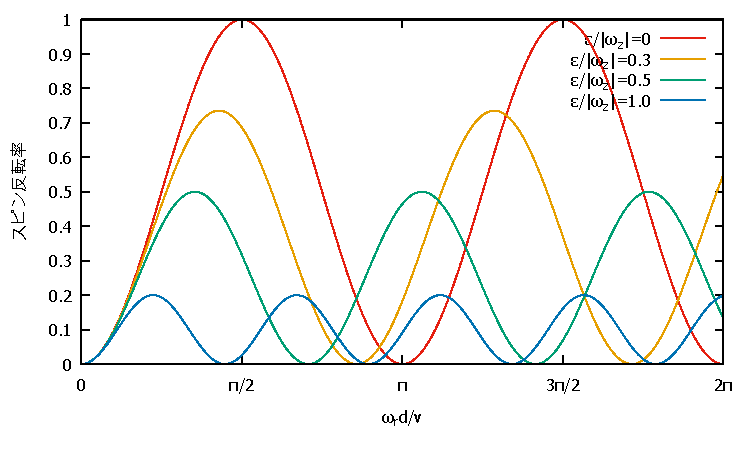
\includegraphics[width=10cm]{resonance/whatwhyhow/resonance_reversalrate.pdf}
\caption{スピン反転率}
\label{Resonance_fig_reversal}
\end{center}
\end{figure}

%\begin{comment}
%\paragraph{振動磁場の反回転成分が無視できる理由}
%略(本の通り)
%\renewcommand{\arraystretch}{1}
%\end{comment}

%\clearpage
\subsection{Why?\ $\sim$スピンフリッパーの共鳴はなぜ必要か$\sim$}
スピンフリッパーの共鳴は本実験での干渉がはっきり見えるかどうかの鍵を握っている。ここではスピンフリッパー共鳴の重要性が明らかとなる。

\paragraph{舞台とあらすじ}
一様磁場中に、理想化されたRFスピンフリッパーふたつとシフタコイルひとつが置かれた状況を考える。系は7つの領域I,II,III,IV,V,VI,VIIからなり、全体に$z$方向一様磁場$B_z$がかけられ、それに加えて領域II,VIに$x$方向振動磁場$2B_r\cos\omega_s t$が、領域IVに$z$方向一様磁場$B$がかけられている。
\begin{figure}[h]
\centering
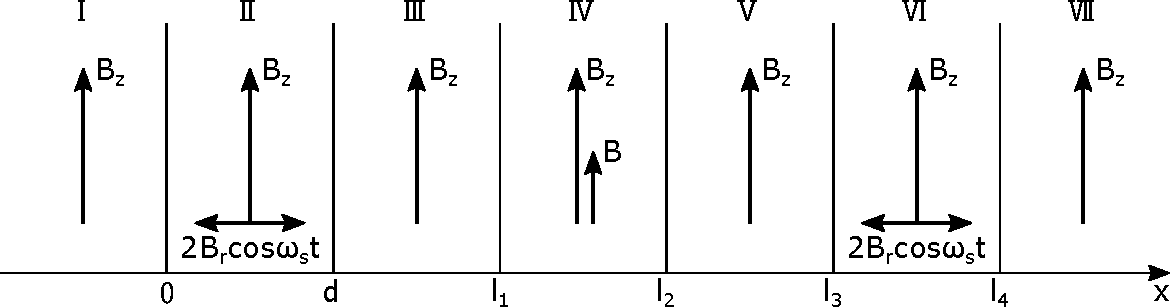
\includegraphics[height=3cm]{resonance/whatwhyhow/Resonance_why_setting.pdf}
\end{figure}

これから述べるように、スピン上向きの中性子が領域Iから入射し、領域I$\sim$VIを通って領域VIIに抜けるとき、領域VIIにおいてスピン上向き中性子を観測する確率は
\begin{equation}
|\psi_\mathrm{VII}^+|^2=N_1(\epsilon)-N_2(\epsilon) \cos (\phi -\Delta(\epsilon)) -N_3(\epsilon) \sin(\phi-\Delta(\epsilon)) \label{Resonance_interference}
\end{equation}
のように書ける。ここで$\epsilon=\omega_s/2-\omega_z$であり、$\phi$はシフタコイル磁場によって生じた位相差、$\Delta(\epsilon)$は$\epsilon$のみに依存した定数位相である。

いま、ある$\epsilon$に対して、シフタコイルの磁場を変えながら領域VIIでのスピン上向き中性子の数を計測すると式(\ref{Resonance_interference})の干渉パターンが得られるが、その見えやすさ(ビジビリティ)は$\epsilon$によって異なる。例えば$N_2/N1=1,N_3/N_1=0$のときは振幅の大きなはっきりとした(ビジビリティの高い)干渉パターンが得られるが、$N_2/N_1,N_3/N_1 \ll 1$のときは干渉パターンはほとんど観測できない(ビジビリティが低い)。ビジビリティを表す指標$V$を
\begin{equation}
V=\sqrt{\left(\frac{N_2}{N_1}\right)^2+\left(\frac{N_3}{N_1}\right)^2}
\end{equation}
で定義すると、$0 \le V \le 1$であり、$V$が大きい程ビジビリティが高い。$\epsilon=0$のとき$V=1$とできることが最後に示される。

すなわちスピンフリッパーを共鳴させる目的は、本実験で得られる干渉パターンのビジビリティを高めるためである。

%\begin{center}(中略)\end{center}


%\begin{comment}
\paragraph{仮定と拝借}
今回は最初から中性子の入射エネルギーはポテンシャルに比べて十分大きいとし、全ての境界で反射は無視する。すると、前節での結果をそのまま拝借することができる。すなわち、領域I,II,IIIにおける波動関数はそれぞれ
\begin{align}
\psi_\mathrm{I}(x,t)&=\begin{pmatrix} 1\\0\end{pmatrix} \e^{i (k_0-\frac{\omega_z}{v})x}\e^{-i\omega_0t}\\
\psi_\mathrm{II}(x,t)&=\begin{pmatrix} \left(\sin^2 \frac{\theta}{2} \e^{i\frac{\omega_A}{v}x} +\cos^2 \frac{\theta}{2} \e^{-i\frac{\omega_A}{v}x} \right) \e^{i(k_0-\frac{\omega_s}{v}) x} \e^{-i\omega_0 t} \\ \sin\frac{\theta}{2}\cos\frac{\theta}{2} \left(\e^{-i\frac{\omega_A}{v}x}-\e^{i\frac{\omega_A}{v}x}\right) \e^{i(k_0-\frac{\omega_s}{v}) x} \e^{-i(\omega_0-\omega_s) t}\end{pmatrix}\\
\psi_\mathrm{III}(x,t)&=\begin{pmatrix} \left(\cos \frac{\omega_A}{v}d +i\frac{\epsilon}{\omega_A} \sin \frac{\omega_A}{v}d\right) \e^{-i\frac{\epsilon}{v} d} \e^{i(k_0-\frac{\omega_z}{v})x}\e^{-i\omega_0t} \\ -i \frac{\omega_r}{\omega_A} \sin \frac{\omega_A}{v}d  \, \e^{i\frac{\epsilon}{v}d} \e^{i(k_0-\frac{\omega_s}{v}+\frac{\omega_z}{v})x}\e^{-i(\omega_0-\omega_s)t} \end{pmatrix}
\end{align}
と書ける。ここで$\epsilon=\omega_s/2-\omega_z,\omega_A=\sqrt{\epsilon^2+\omega_r^2}$であり、$\omega_z=|\mu_n|B_z,\omega_r=|\mu_n|B_r$。$\omega_0$,$v$はそれぞれ中性子の入射エネルギー、速度であり、$k_0=\sqrt{2m\omega_0}$である。その他の記号は前節参照。

\paragraph{領域IV}
領域IVにおけるShr$\ddot{\mathrm{o}}$dinger方程式は
\begin{equation}
i\frac{\del \psi_\mathrm{IV}}{\del t}= \left[-\frac{1}{2m} \frac{\del^2}{\del x^2} +(\omega_z+\omega) \sigma_z\right] \psi_\mathrm{IV}
\end{equation}
ここで$\omega=|\mu_n|B$とした。領域IIIとIVの境界でエネルギーは変化しないので、領域IVにおけるスピン上下成分の波数$k^\pm_\mathrm{IV}$は
\begin{align}
k^+_\mathrm{IV}&=\sqrt{2m(\omega_0-(\omega_z+\omega))}\simeq k_0 -\frac{\omega_z}{v}-\frac{\omega}{v} \\
k^-_\mathrm{IV}&=\sqrt{2m(\omega_0-\omega_s+(\omega_z+\omega))}\simeq k_0 -\frac{\omega_s}{v}+\frac{\omega_z}{v}+\frac{\omega}{v}
\end{align}
となる。反射波を無視し、領域IIIとIVの境界($x=l_1$)で波動関数を接続すると
\begin{equation}
\psi_\mathrm{IV}=\begin{pmatrix} \left(\cos \frac{\omega_A}{v}d +i\frac{\epsilon}{\omega_A} \sin \frac{\omega_A}{v}d\right) \e^{-i\frac{\epsilon}{v} d} \e^{-i\frac{\omega}{v} (x-l_1)} \e^{i(k_0-\frac{\omega_z}{v})x}\e^{-i\omega_0t} \\ -i \frac{\omega_r}{\omega_A} \sin \frac{\omega_A}{v}d  \, \e^{i\frac{\epsilon}{v}d} \e^{i\frac{\omega}{v}(x-l_1)} \e^{i(k_0-\frac{\omega_s}{v}+\frac{\omega_z}{v})x}\e^{-i(\omega_0-\omega_s)t} \end{pmatrix}
\end{equation}
を得る。

\paragraph{領域V}
領域VにおけるShr$\ddot{\mathrm{o}}$dinger方程式は領域I,IIIと等しく、
\begin{equation}
i\frac{\del \psi_\mathrm{V}}{\del t}= \left[-\frac{1}{2m} \frac{\del^2}{\del x^2} +\omega_z \sigma_z\right] \psi_\mathrm{V}
\end{equation}
である。領域VIと同様にして、反射波を無視し、領域IVとVの境界($x=l_2$)で波動関数を接続すると
\begin{equation}
\psi_\mathrm{V}=\begin{pmatrix} \left(\cos \frac{\omega_A}{v}d +i\frac{\epsilon}{\omega_A} \sin \frac{\omega_A}{v}d\right) \e^{-i\frac{\epsilon}{v} d} \e^{-i\frac{\omega}{v} d'} \e^{i(k_0-\frac{\omega_z}{v})x}\e^{-i\omega_0t} \\ -i \frac{\omega_r}{\omega_A} \sin \frac{\omega_A}{v}d  \, \e^{i\frac{\epsilon}{v}d} \e^{i\frac{\omega}{v} d'} \e^{i(k_0-\frac{\omega_s}{v}+\frac{\omega_z}{v})x}\e^{-i(\omega_0-\omega_s)t} \end{pmatrix} \label{Resonance_psi5}
\end{equation}
を得る。ここで$l_2-l_1=d'$を用いた。

\paragraph{領域VI}
領域VIにおける磁場を、領域IIと同じ$z$方向一様磁場と同位相の$x$方向振動磁場
\begin{equation}
\bm{B}_\mathrm{VI}=\hat{\bm{x}}(2B_r)\cos\omega_s t +\hat{\bm{z}}B_z
\end{equation}
とすると、$B_r \ll B_z$のとき
\begin{equation}
\bm{B}_\mathrm{VI} \simeq \hat{\bm{x}} B_r\cos \omega_s t+\hat{\bm{y}} B_r \sin \omega_s t+\hat{\bm{z}} B_z
\end{equation}
と近似でき、前節と同じ議論により領域VIにおける波動関数は次のように書ける:
\begin{equation}
\psi_\mathrm{VI}=\begin{pmatrix} \left(D^+\cos\frac{\theta}{2} \e^{-i\frac{\omega_A}{v} x}-D^-\sin\frac{\theta}{2} \e^{i\frac{\omega_A}{v}x} \right) \e^{i(k_0-\frac{\omega_s}{2v})x} \e^{-i\omega_0 t} \\ \left(D^+\sin\frac{\theta}{2}\e^{-i\frac{\omega_A}{v} x}+D^-\cos\frac{\theta}{2}\e^{i\frac{\omega_A}{v} x}\right) \e^{i(k_0-\frac{\omega_s}{2v})x} \e^{-i(\omega_0-\omega_s) t} \end{pmatrix}
\end{equation}
ここで入射エネルギーは十分大きいとして反射波を無視し、波数を
\begin{equation}
k^\pm_1 =\sqrt{2m\left(\omega_0-\frac{\omega_s}{2}\mp\omega_A\right)} \simeq k_0 -\frac{\omega_s}{2v} \mp\frac{\omega_A}{v}
\end{equation}
と近似した。また、$\cos \theta = -\epsilon/\omega_A,\sin\theta=\omega_r/\omega_A$であり、$D^\pm$は定数である。

\paragraph{領域VとVIの接続}簡単のため式(\ref{Resonance_psi5})で
\begin{align}
\alpha^+ &= \left(\cos \frac{\omega_A}{v}d +i\frac{\epsilon}{\omega_A} \sin \frac{\omega_A}{v}d\right) \e^{-i\frac{\epsilon}{v} d} \e^{-i\frac{\omega}{v} d} \label{Resonance_alpha+}\\
\alpha^-&=-i \frac{\omega_r}{\omega_A} \sin \frac{\omega_A}{v}d  \, \e^{i\frac{\epsilon}{v}d} \e^{i\frac{\omega}{v} d} \label{Resonance_alpha-}
\end{align}
とおき、領域Vでの波動関数を
\begin{equation}
\psi_\mathrm{V} =\begin{pmatrix} \alpha^+ \e^{i(k_0-\frac{\omega_z}{v})x}\e^{-i\omega_0t}\\ \alpha^- \e^{i(k_0-\frac{\omega_s}{v}+\frac{\omega_z}{v})x}\e^{-i(\omega_0-\omega_s)t} \end{pmatrix}
\end{equation}
とかく。領域VとVIの境界($x=l_3$)における接続を考えて、次の2式を得る:
\begin{align}
&\left\{\begin{array}{l} \left(D^+ \cos\frac{\theta}{2} \e^{-i\frac{\omega_A}{v} l_3}-D^-\sin\frac{\theta}{2} \e^{i\frac{\omega_A}{v}l_3}\right) \e^{i(k_0-\frac{\omega_s}{2v})l_3} =\alpha^+ \e^{i(k_0-\frac{\omega_z}{v})l_3} \\ \left(D^+\sin\frac{\theta}{2}\e^{-i\frac{\omega_A}{v} l_3}+D^-\cos\frac{\theta}{2}\e^{i\frac{\omega_A}{v} l_3}\right) \e^{i(k_0-\frac{\omega_s}{2v})l_3} =\alpha^- \e^{i(k_0-\frac{\omega_s}{v}+\frac{\omega_z}{v})l_3}\end{array} \right. \notag \\
&\Rightarrow \left\{\begin{array}{l} D^+ \cos\frac{\theta}{2} \e^{-i\frac{\omega_A}{v} l_3}-D^-\sin\frac{\theta}{2} \e^{i\frac{\omega_A}{v}l_3} =\alpha^+ \e^{i\frac{\epsilon}{v}l_3} \\ D^+\sin\frac{\theta}{2}\e^{-i\frac{\omega_A}{v} l_3}+D^-\cos\frac{\theta}{2}\e^{i\frac{\omega_A}{v} l_3} =\alpha^- \e^{-i\frac{\epsilon}{v}l_3}\end{array} \right. \notag \\
&\Rightarrow \left\{\begin{array}{l} D^+ =\left(\alpha^+ \cos\frac{\theta}{2}\e^{i\frac{\epsilon}{v}l_3} +\alpha^- \sin\frac{\theta}{2}\e^{-i\frac{\epsilon}{v}l_3}\right) \e^{i\frac{\omega_A}{v} l_3} \\ D^-=\left(-\alpha^+ \sin\frac{\theta}{2} \e^{i\frac{\epsilon}{v}l_3} +\alpha^-\cos\frac{\theta}{2}\e^{-i\frac{\epsilon}{v}l_3} \right)\e^{-i\frac{\omega_A}{v} l_3} \end{array} \right.
\end{align}
したがって
\begin{equation}
\psi_\mathrm{VI} =\left( \begin{array}{l} \left[\alpha^+ \left(\cos^2\frac{\theta}{2}\e^{-i\frac{\omega_A}{v}(x-l_3)} +\sin^2\frac{\theta}{2}\e^{i\frac{\omega_A}{v}(x-l_3)} \right)\e^{i\frac{\epsilon}{v}l_3} \right. \\ \hspace{2cm}\left. +\alpha^- \sin\frac{\theta}{2}\cos\frac{\theta}{2} \left(\e^{-i\frac{\omega_A}{v}(x-l_3)}-\e^{i\frac{\omega_A}{v}(x-l_3)}\right)\e^{-i\frac{\epsilon}{v}l_3}\right]\e^{i(k_0-\frac{\omega_s}{2v})x}\e^{-\omega_0t} \\ \left[\alpha^+ \sin\frac{\theta}{2}\cos\frac{\theta}{2} \left(\e^{-i\frac{\omega_A}{v}(x-l_3)}-\e^{i\frac{\omega_A}{v}(x-l_3)}\right)\e^{i\frac{\epsilon}{v}l_3} \right. \\ \hspace{2cm} \left. +\alpha^- \left(\sin^2\frac{\theta}{2}\e^{-i\frac{\omega_A}{v}(x-l_3)} +\cos^2\frac{\theta}{2}\e^{i\frac{\omega_A}{v}(x-l_3)} \right) \e^{-i\frac{\epsilon}{v}l_3}\right] \e^{i(k_0-\frac{\omega_s}{2v})x} \e^{-i(\omega_0-\omega_s) t} \end{array}\right)
\end{equation}
となる。

\paragraph{領域VII}
領域VにおけるShr$\ddot{\mathrm{o}}$dinger方程式は領域I,III,Vと同じく
\begin{equation}
i\frac{\del \psi_\mathrm{VII}}{\del t}= \left[-\frac{1}{2m} \frac{\del^2}{\del x^2} +\omega_z \sigma_z\right] \psi_\mathrm{VII}
\end{equation}
であり、領域VIとVIIの境界($x=l_4$)で波動関数を接続すると次式を得る:
\begin{align}
\psi_\mathrm{VII} &=\left( \begin{array}{l} \left[\alpha^+ \left(\cos^2\frac{\theta}{2}\e^{-i\frac{\omega_A}{v}(l_4-l_3)} +\sin^2\frac{\theta}{2}\e^{i\frac{\omega_A}{v}(l_4-l_3)} \right)\e^{i\frac{\epsilon}{v}l_3} \right. \\ \hspace{1cm}\left. +\alpha^- \sin\frac{\theta}{2}\cos\frac{\theta}{2} \left(\e^{-i\frac{\omega_A}{v}(l_4-l_3)}-\e^{i\frac{\omega_A}{v}(l_4-l_3)}\right)\e^{-i\frac{\epsilon}{v}l_3}\right]\e^{i(k_0-\frac{\omega_s}{2v})l_4} \e^{i(k_0-\frac{\omega_z}{v})(x-l_4)} \e^{-\omega_0t} \\ \left[\alpha^+ \sin\frac{\theta}{2}\cos\frac{\theta}{2} \left(\e^{-i\frac{\omega_A}{v}(l_4-l_3)}-\e^{i\frac{\omega_A}{v}(l_4-l_3)}\right)\e^{i\frac{\epsilon}{v}l_3} \right. \\ \hspace{1cm} \left. +\alpha^- \left(\sin^2\frac{\theta}{2}\e^{-i\frac{\omega_A}{v}(l_4-l_3)} +\cos^2\frac{\theta}{2}\e^{i\frac{\omega_A}{v}(l_4-l_3)} \right) \e^{-i\frac{\epsilon}{v}l_3}\right] \e^{i(k_0-\frac{\omega_s}{2v})l_4} \e^{i(k_0-\frac{\omega_s}{v}+\frac{\omega_z}{v})(x-l_4)} \e^{-i(\omega_0-\omega_s) t} \end{array}\right) \notag \\
&=\left( \begin{array}{l} \left[\alpha^+ \left(\cos^2\frac{\theta}{2}\e^{-i\frac{\omega_A}{v}d} +\sin^2\frac{\theta}{2}\e^{i\frac{\omega_A}{v}d} \right)\e^{i\frac{\epsilon}{v}l_3} \right. \\ \hspace{2cm}\left. +\alpha^- \sin\frac{\theta}{2}\cos\frac{\theta}{2} \left(\e^{-i\frac{\omega_A}{v}d}-\e^{i\frac{\omega_A}{v}d}\right)\e^{-i\frac{\epsilon}{v}l_3}\right]\e^{-i\frac{\epsilon}{v}l_4}\e^{i(k_0-\frac{\omega_z}{v})x} \e^{-\omega_0t} \\ \left[\alpha^+ \sin\frac{\theta}{2}\cos\frac{\theta}{2} \left(\e^{-i\frac{\omega_A}{v}d}-\e^{i\frac{\omega_A}{v}d}\right)\e^{i\frac{\epsilon}{v}l_3} \right. \\ \hspace{2cm} \left. +\alpha^- \left(\sin^2\frac{\theta}{2}\e^{-i\frac{\omega_A}{v}d} +\cos^2\frac{\theta}{2}\e^{i\frac{\omega_A}{v}d} \right) \e^{-i\frac{\epsilon}{v}l_3}\right] \e^{i\frac{\epsilon}{v}l_4} \e^{i(k_0-\frac{\omega_s}{v}+\frac{\omega_z}{v})x} \e^{-i(\omega_0-\omega_s) t} \end{array}\right)
\end{align}
ここで$l_4-l_3=d$を用いた。さらに$\cos\theta=-\epsilon/\omega_A,\sin\theta=\omega_r/\omega_A$より
\begin{align}
&\cos^2 \frac{\theta}{2} \e^{-i\frac{\omega_A}{v}d} +\sin^2 \frac{\theta}{2} \e^{i\frac{\omega_A}{v}d} =\cos \frac{\omega_A}{v}d +i\frac{\epsilon}{\omega_A} \sin \frac{\omega_A}{v}d \\
&\sin^2 \frac{\theta}{2} \e^{-i\frac{\omega_A}{v}d} +\cos^2 \frac{\theta}{2} \e^{i\frac{\omega_A}{v}d} =\left(\cos^2 \frac{\theta}{2} \e^{-i\frac{\omega_A}{v}d} +\sin^2 \frac{\theta}{2} \e^{i\frac{\omega_A}{v}d}\right)^\dagger=\cos \frac{\omega_A}{v}d -i\frac{\epsilon}{\omega_A} \sin \frac{\omega_A}{v}d \\
&\sin\frac{\theta}{2}\cos\frac{\theta}{2} \left(\e^{-i\frac{\omega_A}{v}d}-\e^{i\frac{\omega_A}{v}d}\right) = -i \frac{\omega_r}{\omega_A} \sin \frac{\omega_A}{v}d
\end{align}
を用い、(\ref{Resonance_alpha+}),(\ref{Resonance_alpha-})の$\alpha^\pm$を代入して
\begin{align}
\psi_\mathrm{VII} &= \left( \begin{array}{l} \left[\left(\cos \frac{\omega_A}{v}d +i\frac{\epsilon}{\omega_A} \sin \frac{\omega_A}{v}d\right)^2\e^{i\frac{\epsilon}{v}(l_3-d)}\e^{-i\frac{\omega}{v}d'} \right. \\ \hspace{2cm}\left. +\left(-i \frac{\omega_r}{\omega_A} \sin \frac{\omega_A}{v}d\right)^2\e^{-i\frac{\epsilon}{v}(l_3-d)}\e^{i\frac{\omega}{v}d'} \right]\e^{-i\frac{\epsilon}{v}l_4}\e^{i(k_0-\frac{\omega_z}{v})x} \e^{-\omega_0t} \\ \left[\left(\cos \frac{\omega_A}{v}d +i\frac{\epsilon}{\omega_A} \sin \frac{\omega_A}{v}d\right) \left(-i \frac{\omega_r}{\omega_A} \sin \frac{\omega_A}{v}d\right) \e^{i\frac{\epsilon}{v}(l_3-d)}\e^{-i\frac{\omega}{v}d'} \right. \\ \hspace{1cm} \left. +\left(-i \frac{\omega_r}{\omega_A} \sin \frac{\omega_A}{v}d\right) \left(\cos \frac{\omega_A}{v}d -i\frac{\epsilon}{\omega_A} \sin \frac{\omega_A}{v}d\right) \e^{-i\frac{\epsilon}{v}(l_3-d)}\e^{i\frac{\omega}{v}d'} \right] \e^{i\frac{\epsilon}{v}l_4} \e^{i(k_0-\frac{\omega_s}{v}+\frac{\omega_z}{v})x} \e^{-i(\omega_0-\omega_s) t} \end{array}\right) \notag \\
&=\left( \begin{array}{l} \left[\left(\cos \frac{\omega_A}{v}d +i\frac{\epsilon}{\omega_A} \sin \frac{\omega_A}{v}d\right)^2\e^{i\frac{\epsilon}{v}L'}\e^{-i\frac{\omega}{v}d'} \right. \\ \hspace{2cm}\left. +\left(-i \frac{\omega_r}{\omega_A} \sin \frac{\omega_A}{v}d\right)^2\e^{-i\frac{\epsilon}{v}L'}\e^{i\frac{\omega}{v}d'} \right]\e^{-i\frac{\epsilon}{v}L}\e^{i(k_0-\frac{\omega_z}{v})x} \e^{-\omega_0t} \\ \left(-i \frac{\omega_r}{\omega_A} \sin \frac{\omega_A}{v}d\right) \left[\left(\cos \frac{\omega_A}{v}d +i\frac{\epsilon}{\omega_A} \sin \frac{\omega_A}{v}d\right) \e^{i\frac{\epsilon}{v}L'}\e^{-i\frac{\omega}{v}d'} \right. \\ \hspace{2cm} \left. +\left(\cos \frac{\omega_A}{v}d -i\frac{\epsilon}{\omega_A} \sin \frac{\omega_A}{v}d\right) \e^{-i\frac{\epsilon}{v}L'}\e^{i\frac{\omega}{v}d'} \right] \e^{i\frac{\epsilon}{v}L} \e^{i(k_0-\frac{\omega_s}{v}+\frac{\omega_z}{v})x} \e^{-i(\omega_0-\omega_s) t} \end{array}\right)
\end{align}
となる。ここで$l_3-d=L',l_4=L$とした。
%\end{comment}


\paragraph{結末}
以上のようにして、領域Iで
\begin{equation}
\psi_\mathrm{I}(x,t)=\begin{pmatrix} 1\\0\end{pmatrix} \e^{i (k_0-\frac{\omega_z}{v})x}\e^{-i\omega_0t}
\end{equation}
と表された入射中性子は領域II$\sim$VIを通って領域VIIで
\begin{equation}
\psi_\mathrm{VII}(x,t) =\left( \begin{array}{l} \left[\left(\cos \frac{\omega_A}{v}d +i\frac{\epsilon}{\omega_A} \sin \frac{\omega_A}{v}d\right)^2\e^{i\frac{\epsilon}{v}L'}\e^{-i\frac{\omega}{v}d'} \right. \\ \hspace{2cm}\left. +\left(-i \frac{\omega_r}{\omega_A} \sin \frac{\omega_A}{v}d\right)^2\e^{-i\frac{\epsilon}{v}L'}\e^{i\frac{\omega}{v}d'} \right]\e^{-i\frac{\epsilon}{v}L}\e^{i(k_0-\frac{\omega_z}{v})x} \e^{-\omega_0t} \\ \left(-i \frac{\omega_r}{\omega_A} \sin \frac{\omega_A}{v}d\right) \left[\left(\cos \frac{\omega_A}{v}d +i\frac{\epsilon}{\omega_A} \sin \frac{\omega_A}{v}d\right) \e^{i\frac{\epsilon}{v}L'}\e^{-i\frac{\omega}{v}d'} \right. \\ \hspace{2cm} \left. +\left(\cos \frac{\omega_A}{v}d -i\frac{\epsilon}{\omega_A} \sin \frac{\omega_A}{v}d\right) \e^{-i\frac{\epsilon}{v}L'}\e^{i\frac{\omega}{v}d'} \right] \e^{i\frac{\epsilon}{v}L} \e^{i(k_0-\frac{\omega_s}{v}+\frac{\omega_z}{v})x} \e^{-i(\omega_0-\omega_s) t} \end{array}\right)
\end{equation}
という状態をとることがわかった。したがって、領域VIIでスピン上向き中性子を観測する確率は
\begin{align}
|\psi_\mathrm{VII}^+|^2&=\Biggl| \left(\cos \frac{\omega_A}{v}d +i\frac{\epsilon}{\omega_A} \sin \frac{\omega_A}{v}d\right)^2\e^{i\frac{\epsilon}{v}L'}\e^{-i\frac{\omega}{v}d'} +\left(-i \frac{\omega_r}{\omega_A} \sin \frac{\omega_A}{v}d\right)^2\e^{-i\frac{\epsilon}{v}L'}\e^{i\frac{\omega}{v}d'} \Biggr|^2 \notag \\
&=\left[\left(\cos \frac{\omega_A}{v}d +i\frac{\epsilon}{\omega_A} \sin \frac{\omega_A}{v}d\right)^2\e^{i\frac{\epsilon}{v}L'}\e^{-i\frac{\omega}{v}d'} +\left(-i \frac{\omega_r}{\omega_A} \sin \frac{\omega_A}{v}d\right)^2\e^{-i\frac{\epsilon}{v}L'}\e^{i\frac{\omega}{v}d'}\right] \notag\\
&\hspace{2cm} \times \left[\left(\cos \frac{\omega_A}{v}d -i\frac{\epsilon}{\omega_A} \sin \frac{\omega_A}{v}d\right)^2\e^{-i\frac{\epsilon}{v}L'}\e^{i\frac{\omega}{v}d'} +\left(i \frac{\omega_r}{\omega_A} \sin \frac{\omega_A}{v}d\right)^2\e^{i\frac{\epsilon}{v}L'}\e^{-i\frac{\omega}{v}d'}\right] \notag \\
&=\left(\cos^2 \frac{\omega_A}{v}d +\left(\frac{\epsilon}{\omega_A}\right)^2 \sin^2 \frac{\omega_A}{v}d\right)^2+\left(\frac{\omega_r}{\omega_A}\right)^4 \sin^4 \frac{\omega_A}{v}d \notag \\
&\hspace{1cm}  -2\left(\frac{\omega_r}{\omega_A}\right)^2\sin^2\frac{\omega_A}{v}d \left[\left(\cos^2 \frac{\omega_A}{v}d -\left(\frac{\epsilon}{\omega_A}\right)^2 \sin^2 \frac{\omega_A}{v}d\right) \cos \left(\frac{2}{v}(\omega d'-\epsilon L')\right) \right. \notag \\
&\hspace{6.3cm} \left.+2 \frac{\epsilon}{\omega_A} \sin \frac{\omega_A}{v}d \cos \frac{\omega_A}{v}d \sin \left(\frac{2}{v}(\omega d'-\epsilon L')\right)\right]
\end{align}
となる。
\begin{align}
&N_1 = \left(\cos^2 \frac{\omega_A}{v}d +\left(\frac{\epsilon}{\omega_A}\right)^2 \sin^2 \frac{\omega_A}{v}d\right)^2+\left(\frac{\omega_r}{\omega_A}\right)^4 \sin^4 \frac{\omega_A}{v}d \\
&N_2 = 2\left(\frac{\omega_r}{\omega_A}\right)^2\sin^2\frac{\omega_A}{v}d \left(\cos^2 \frac{\omega_A}{v}d -\left(\frac{\epsilon}{\omega_A}\right)^2 \sin^2 \frac{\omega_A}{v}d\right) \\
&N_3 = 4\frac{\epsilon}{\omega_A} \left(\frac{\omega_r}{\omega_A}\right)^2\sin^3\frac{\omega_A}{v}d \cos \frac{\omega_A}{v}d
\end{align}
とおけばこれを
\begin{equation}
|\psi_\mathrm{VII}^+|^2 =N_1 -N_2 \cos \left(\frac{2}{v}(\omega d'-\epsilon L')\right)-N_3 \sin  \left(\frac{2}{v}(\omega d'-\epsilon L')\right) \label{Resonance_interference2}
\end{equation}
と書くことができる。

いま、ある$\epsilon$に対して、シフタコイルの磁場を変えながら領域VIIでのスピン上向き中性子の数を計測すると式(\ref{Resonance_interference2})の干渉パターンが得られるが、その見えやすさ(ビジビリティ)は$\epsilon$によって異なる。例えば$N_2/N_1=1,N_3/N_1=0$のときは振幅の大きなはっきりとした(ビジビリティの高い)干渉パターンが得られるが、$N_2/N_1,N_3/N_1 \ll 1$のときは干渉パターンはほとんど観測できない(ビジビリティが低い)。ビジビリティを表す指標$V$を
\begin{equation}
V=\sqrt{\left(\frac{N_2}{N_1}\right)^2+\left(\frac{N_3}{N_1}\right)^2}
\end{equation}
で定義すると
\begin{equation}
V=\frac{2\left(\frac{\omega_r}{\omega_A}\right)^2\sin^2\frac{\omega_A}{v}d \left(\cos^2 \frac{\omega_A}{v}d+\left(\frac{\epsilon}{\omega_A}\right)^2\sin^2\frac{\omega_A}{v}d\right)}{\left(\cos^2 \frac{\omega_A}{v}d+\left(\frac{\epsilon}{\omega_A}\right)^2\sin^2\frac{\omega_A}{v}d\right)^2+\left(\frac{\omega_r}{\omega_A}\right)^4\sin^4\frac{\omega_A}{v}d}
\end{equation}
となるから$0 \le V \le 1$であり、$V$が大きい程ビジビリティが高い。

\begin{comment}
ここで$\Omega_A = \omega_A d/v,\Omega_r= \omega_r d/v,\mathcal{E}=\epsilon d/v,\Omega=\omega d'/v,\mathcal{L}'=L'/d$と無次元化すると
\begin{align}
&N_1 = \left(\cos^2 \Omega_A +\left(\frac{\mathcal{E}}{\Omega_A}\right)^2 \sin^2 \Omega_A \right)^2+\left(\frac{\Omega_r}{\Omega_A}\right)^4 \sin^4 \frac{\Omega_A}{v}d \\
&N_2 = 2\left(\frac{\Omega_r}{\Omega_A}\right)^2\sin^2\Omega_A \left(\cos^2 \Omega_A -\left(\frac{\mathcal{E}}{\Omega_A}\right)^2 \sin^2 \Omega_A\right) \\
&N_3 = 4\frac{\mathcal{E}}{\Omega_A} \left(\frac{\Omega_r}{\Omega_A}\right)^2\sin^3\Omega_A \cos \Omega_A \\
&|\psi_\mathrm{VII}|^2 =N_1 -N_2 \cos 2(\Omega-\mathcal{E} \mathcal{L}')-N_3 \sin 2(\Omega -\mathcal{E} \mathcal{L}')
\end{align}
\end{comment}

\begin{comment}
ここで$E=\epsilon d/v$と無次元化し、$\omega_rd/v=\pi/4$のときの$E$と$V$の関係を図示すると図\ref{Resonance_fig_visivility}のようになる。$E=0$のとき$V=1$となり、ビジビリティが最高となることがわかる。また$-0.2 \le E \le 0.2$でも$V \simeq 1$でビジビリティは十分高い。実際、$\omega_rd/v=\pi/4$,$E=0,0.2,0.5,1,2$のときに$\Omega=\omega d'/v$と$|\psi_\mathrm{VII}|^2$の関係を図示すると図\ref{Resonance_fig_interference}のようになる。ただし$L'/d=10$とした。
\end{comment}

いま$\omega_r/\omega_z=0.25$とし、$\epsilon/\omega_z=0,0.3,0.5,1.0$の各場合について干渉パターンのビジビリティ$V$と$\omega_r d/v$の関係を図\ref{Resonance_fig_visivility}に表す。図\ref{Resonance_fig_visivility}より共鳴条件
$
\epsilon=\frac{\omega_s}{2}-\omega_z=0 \label{Resonance_resonance}
$
がなりたてば、$\omega_r d/v =(2n+1)\pi/4 \ (n =0,1,2,\cdots)$を満たす速度の中性子に対して、干渉パターンのビジビリティ$V=1$になることがわかる。逆に$\epsilon \neq 0$のときはどのような速度の中性子に対してもビジビリティは1となり得ない。実際、$\omega_rd/v=\pi/4$,$\epsilon/\omega_z=0,0.3,0.5,1.0$のときに$\chi=\omega d'/v$と$|\psi_\mathrm{VII}|^2$の関係を図示すると図\ref{Resonance_fig_interference}のようになる。ただし$L'/d=10$とした。

\begin{figure}[h]
%\begin{minipage}{0.5\hsize}
\begin{center}
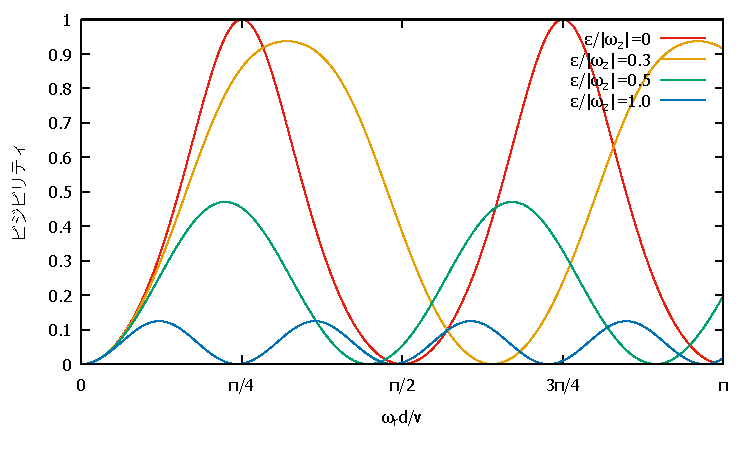
\includegraphics[width=10cm]{resonance/whatwhyhow/resonance_visivility1.pdf}
\caption{ビジビリティ}
\label{Resonance_fig_visivility}
%\end{center}
%\end{minipage}
%\begin{minipage}{0.5\hsize}
%\begin{center}
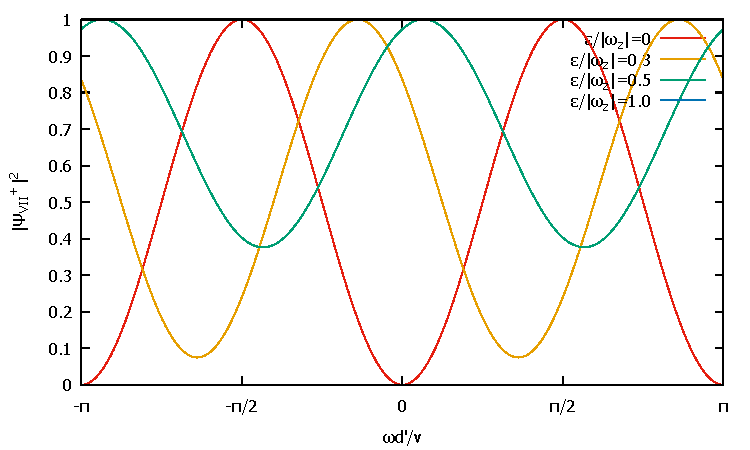
\includegraphics[width=10cm]{resonance/whatwhyhow/resonance_interference1.pdf}
\caption{干渉}
\label{Resonance_fig_interference}
\end{center}
%\end{minipage}
\end{figure}

すなわちスピンフリッパーを共鳴させる目的は、実験で得られる干渉パターンのビジビリティを高めるためである。
\renewcommand{\arraystretch}{1}

\clearpage
\subsection{How?\ $\sim$スピンフリッパーを共鳴させるには$\sim$}
実際にスピンフリッパーを共鳴させるにはどうしたらよいだろう。ここではその実現方法を考え、実際に実験で用いた装置と従った手順を紹介する。

\paragraph{実現方法}
\ref{Resonance_what}節と同じく、一様磁場中にスピンフリッパーがひとつ置かれており、スピン上向き中性子を領域Iから入射させる場合を考える。このとき領域IIIでスピン上向き中性子を観測する確率は式(\ref{Resonance_1-reversal})より
\begin{equation}
\bigl|\psi_\mathrm{III}^+\bigr|^2 =\cos^2 \frac{\omega_A}{v}d+\left(\frac{\epsilon}{\omega_A}\right)^2\sin^2\frac{\omega_A}{v}d
\end{equation}
であらわされる。これを$\omega_r/\omega_z=0.5$のときに、$\epsilon/\omega_z=0,0.3,0.5,1.0$の各場合について$\omega_r d/v$に対して図示すると図\ref{Resonance_fig_1-reversal}のようになる。図\ref{Resonance_fig_1-reversal}より、領域IIIでスピン上向き中性子を観測する確率の、速度に対する最小値は共鳴条件(\ref{Resonance_resonance2})
\[
\epsilon=\frac{\omega_s}{2}-\omega_z=0
\]
を満たすとき最も小さくなり、理想的にはゼロとなることがわかる。共鳴条件を満たすときに領域IIIでスピン上向き中性子を観測する確率がゼロとなるための速度に対する条件
\begin{equation}
\frac{\omega_rd}{v}=\frac{\pi}{2}
\end{equation}
を$\pi$フリップ条件と呼ぶ。
\begin{figure}[h]
\begin{center}
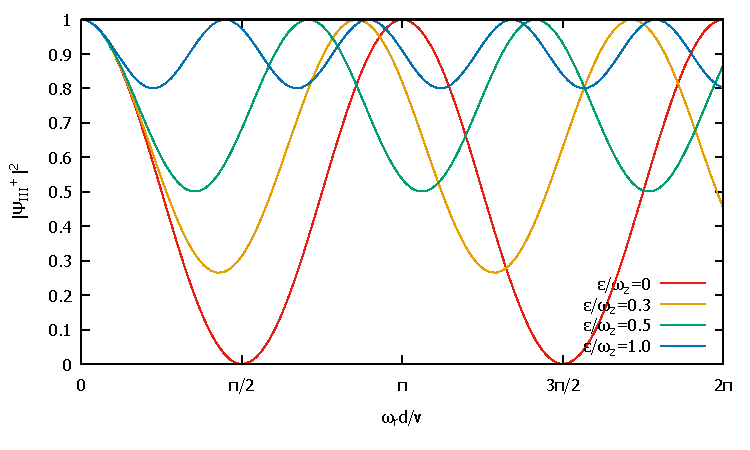
\includegraphics[width=10cm]{resonance/whatwhyhow/resonance_1-reversal.pdf}
\caption{$1-反転率$}
\label{Resonance_fig_1-reversal}
\end{center}
\end{figure}

すなわち次のようにして、実験的にスピンフリッパーの共鳴を実現することができる。
\begin{enumerate}
\item スピンフリッパーにスピン上向き中性子を入射し、フリッパーの後ろでスピン上向き成分のみを観測する。
\item 共鳴条件が満たされていないと、ある速度の中性子についてはカウントをより減らすことができる。
\item 共鳴条件が満たされていると、$\pi$フリップ条件を満たす速度の中性子についてはスピンが完全に反転するため、その速度の中性子のカウントは最小となる。
\item カウント分布を見ながら共鳴条件に関するパラメータを調節し、カウントが最小となるところを探す。
\end{enumerate}


\paragraph{実験装置}
上流側、下流側それぞれのスピンフリッパーに対して共鳴実験を行った。用いた装置は
\vspace{5mm}
\begin{minipage}{0.5\hsize}
\begin{enumerate}
\item 上流側スピンフリッパー共鳴実験
\begin{enumerate}
\item ガイド磁場コイル
\item 上流側中性子磁気スーパーミラー
\item[(c1)] 上流側スピンフリッパー
\setcounter{enumii}{3}
\item 下流側中性子磁気スーパーミラー
\item \ce{^3He}ガスを充填した比例計数管
\end{enumerate}
\end{enumerate}
\end{minipage}
\begin{minipage}{0.5\hsize}
\begin{enumerate}
\setcounter{enumi}{1}
%\renewcommand{\labelenumi}{}
\item 下流側スピンフリッパー共鳴実験
\begin{enumerate}
\item ガイド磁場コイル
\item 上流側中性子磁気スーパーミラー
%\renewcommand{\labelenumi}{(\alph{enumi} {2})}
\item[(c2)] 下流側スピンフリッパー
\setcounter{enumii}{3}
%\renewcommand{\labelenumi}{(\alph{enumi})}
\item 下流側中性子磁気スーパーミラー
\item \ce{^3He}ガスを充填した比例計数管
\end{enumerate}
\end{enumerate}
\end{minipage}
\vspace{5mm}

また、回路系には次の機器を用い、図のように接続した。
\begin{enumerate}
\renewcommand{\labelenumi}{(\roman{enumi})}
\item 直流安定化電源PWX750MLF(KIKUSUI) $\times 3$ \ \ (以後、直流電源1,2,3)
\item マルチファンクションジェネレータWF1974(エヌエフ回路設計ブロック) \ \ (以後、FG)
\item 1MHzバイポーラ電源HSA4014(エヌエフ回路設計ブロック) $\times 2$ \ \ (以後、アンプ1,2)
\end{enumerate}

\vspace{1cm}
\begin{figure}[h]
\centering
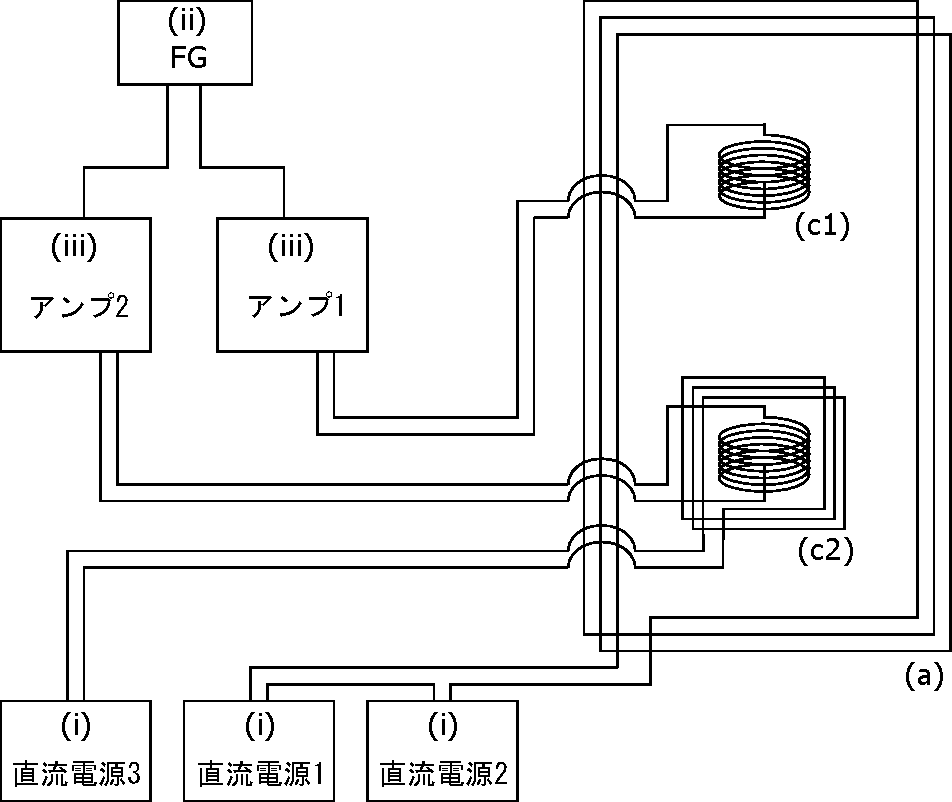
\includegraphics[width=12cm]{resonance/whatwhyhow/kairozu.pdf}
\caption{配線図}
\end{figure}

\clearpage
\paragraph{実験手順}
実験は次のフローチャートに沿って行った。
\begin{figure}[h]
\centering
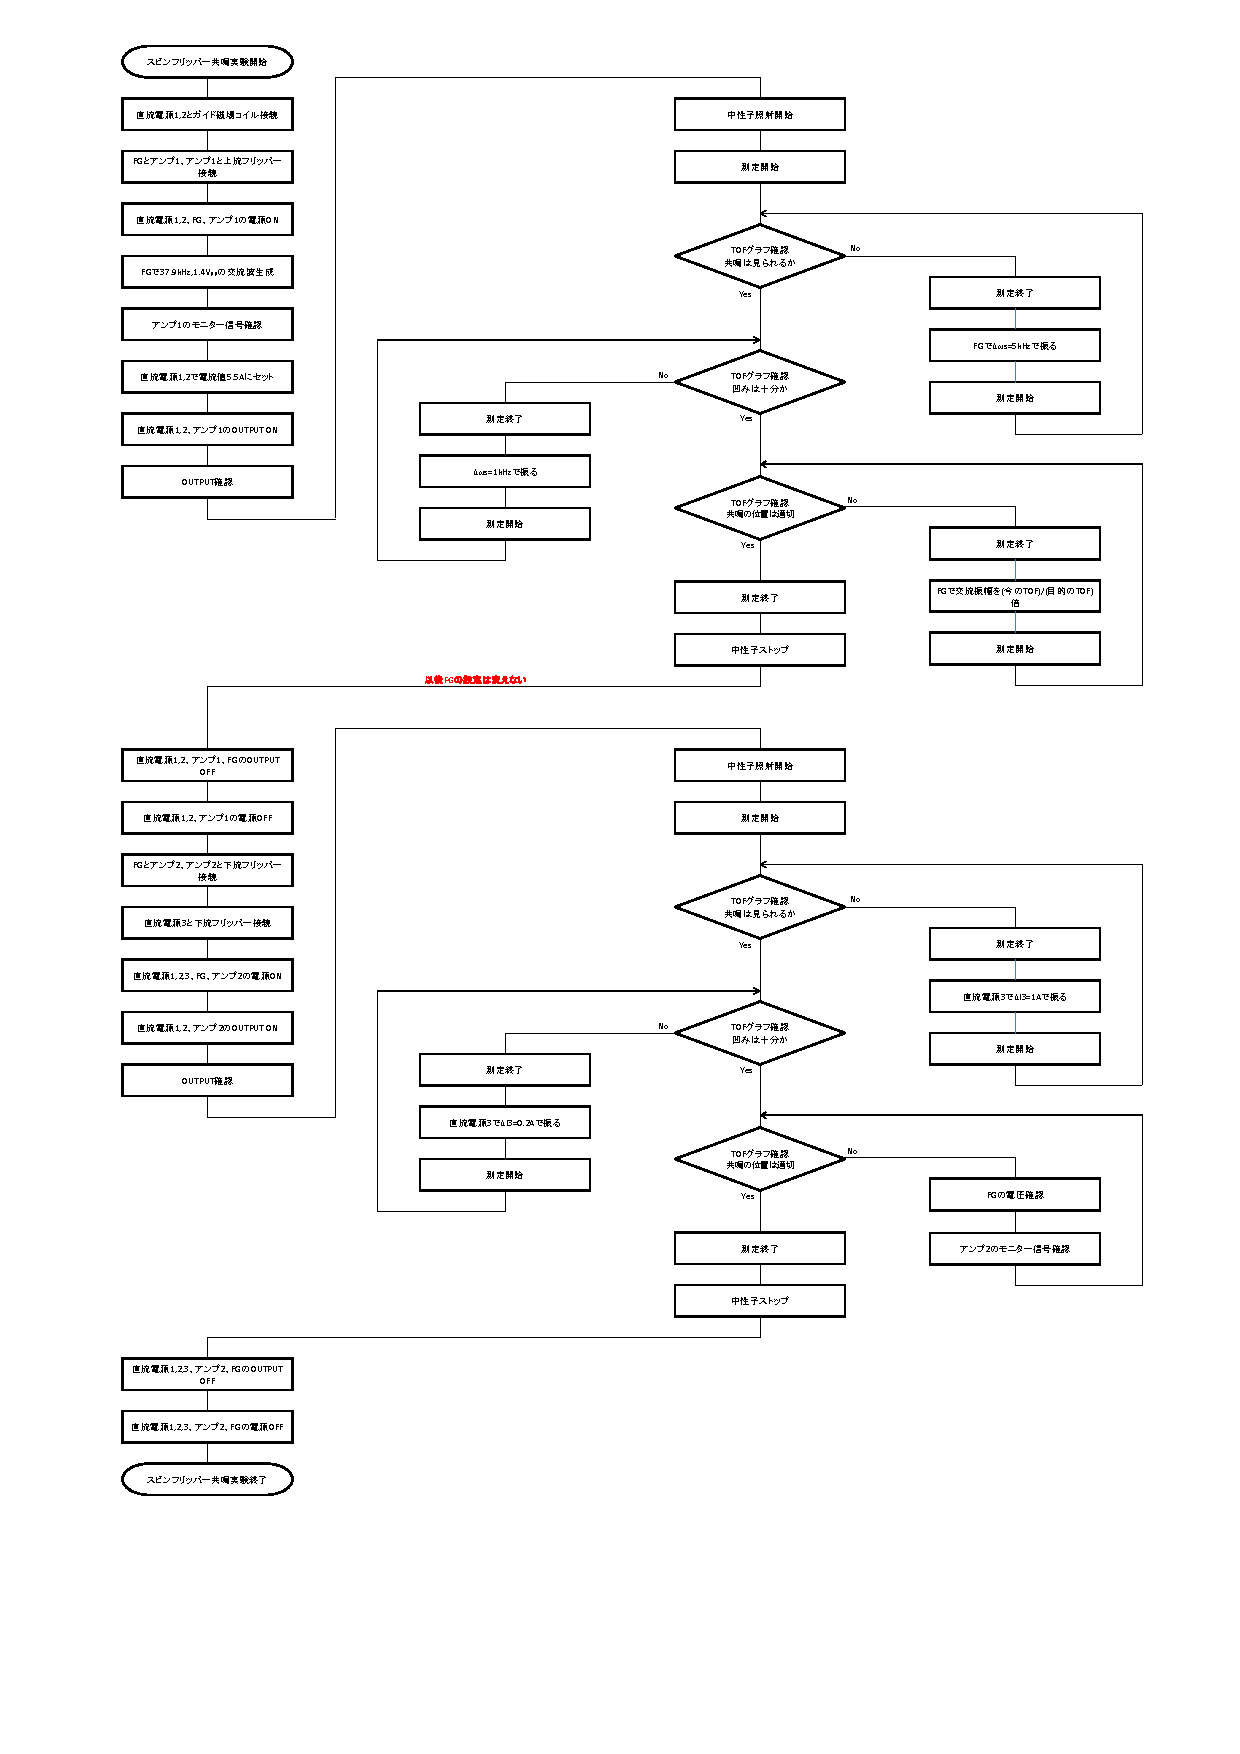
\includegraphics[width=\hsize]{resonance/whatwhyhow/Resonance_flow.pdf}
\vspace{-3.5cm}
\end{figure}

\newpage
次は実際の実験手順である。
\begin{enumerate}
%\renewcommand{\labelenumi}{\arabic{enumi})}
\item (2017.2.22)装置、機器を図のとおりに配置、接続し、上流フリッパー共鳴実験を開始した。
\item 直流電源1,2でガイド磁場コイルに5.5Aの電流を流した。
\item FGで周波数$37.9\, \mathrm{kHz},振幅14.0\, \mathrm{V_{pp}}$の交流波を生成し、アンプ1で増幅して上流フリッパーに交流電流を流した。
\item 中性子の照射を開始した。
\item 測定を開始した。
\item 10分程度データを取り、TOF分布に凹みを確認した。
\item FGで交流波の周波数を$37.0,38.8,36.0,34.0,41.0,40.0 \, \mathrm{kHz}$と変えながら、それぞれ10分程度データを収集した。
\item データ収集と平行して解析を行い、交流波の周波数を$37.5\, \mathrm{kHz}$,振幅を$14.0\, \mathrm{V_{pp}}$に決定した。
\item 中性子照射をストップし、機器の電源を落として上流フリッパー共鳴実験を終了した。
\item (2017.2.23)装置、機器を図のとおりに配置、接続し、下流フリッパー共鳴実験を開始した。
\item 直流電源1,2でガイド磁場コイルに5.5Aの電流を流した。
\item FGで周波数$37.5\, \mathrm{kHz},振幅14.0\, \mathrm{V_{pp}}$の交流波を生成し、アンプ2で増幅して下流フリッパーに交流電流を流した。
\item 中性子の照射を開始した。
\item 測定を開始した。
\item 10分程度データを取り、TOF分布に凹みを確認した。
\item 直流電源3でガイド磁場補正用コイルに流す電流を$0.1,0.5,0.3\,\mathrm{A}$と変えながら、それぞれ10分程度データを収集した。
\item 一旦中性子照射をストップし直流電源3をガイド磁場補正用コイルに逆向きにつなぎ替え、再び中性子照射を開始した。
\item 直流電源3でガイド磁場補正用コイルに流す電流を$-1.0,-0.5,-2.0\,\mathrm{A}$と変えながら、それぞれ10分程度データを収集した。
\item 一旦中性子照射をストップし直流電源3をガイド磁場補正用コイルに逆向きにつなぎ替え、再び中性子照射を開始した。
\item 直流電源3でガイド磁場補正用コイルに流す電流を$1.0,2.0\,\mathrm{A}$と変えて、それぞれ10分程度データを収集した。
\item データ収集と平行して解析を行い、ガイド磁場補正用コイルの電流値を$0.185\,\mathrm{A}$に決定した。
\item 中性子照射をストップし、機器の電源を落として下流フリッパー共鳴実験を終了した。
\end{enumerate}

\begin{itemize}
\item[(注$\!\!$1)] ガイド磁場コイル、ガイド磁場補正用コイルに流す電流は、電流を流したときに鉛直下向きの磁場が発生する向きを正とした。
\item[(注$\!\!$2)] 下流フリッパー共鳴実験中、ガイド磁場コイルが接触不良のためうまく機能せず正しいデータが取れない事態が発生したが、それについては省略した。
\end{itemize}

%\newpage
\paragraph{パラメータ初期設定}
スピンフリッパー共鳴実験で実際に制御できるパラメータはFGで生成する交流電圧の周波数$f_s$,振幅$V_r$と直流電源3で下流フリッパーのガイド磁場補正用コイルに流す電流$I_c$の3つである。実験は共鳴条件と$\pi$フリップ条件を満たすようにこれらを適当に変えながら進めたが、初期設定としてこれらの値をある程度正確に決めておく必要がある。なぜなら、もし最初に全く共鳴が見えないと、どのパラメータをどの程度動かしてよいか全く見当がつかないから。

スピンフリッパーにかける振動磁場の角振動数$\omega_s$と振幅$2B_r$の2つのは、それぞれフリッパーが置かれた場所におけるガイド磁場コイルの磁場$B_z$とターゲットとする中性子の速度$v$から定まる。すなわち$\omega_s$は共鳴条件(\ref{Resonance_resonance})より
\begin{equation}
\omega_s = 2\omega_z =2 |\mu_n|B_z
\end{equation}
$B_r$は$\pi$フリップ条件より
\begin{equation}
2B_r =\frac{2 \omega_r}{|\mu_n|} =\frac{\pi v}{|\mu_n|d}
\end{equation}
で定まる。

$B_z$としてはシミュレーションと実測より$B_z=13 \, \mathrm{G}$を、$v$としてはフリッパー無しのときの速度分布である程度カウントの多かった$v=1000\, \mathrm{m/s}$を入れてそれぞれ計算すると
\begin{equation}
\omega_s/2\pi\simeq 37.9\, \mathrm{kHz}, \quad B_r\simeq 5.7 \, \mathrm{G}
\end{equation}
を得る。従ってFGで生成する交流電圧の周波数$f_s$の初期値は$37.9\,\mathrm{kHz}$と決めた。

また、フリッパーを直径90mm幅30mmの30巻きソレノイドコイルとして、1Aの電流を流したときの中心での磁場の大きさ$b_f$[G]と、37.9kHzの交流電圧をかけたときのインピーダンス$Z[\Omega]$を計算するとそれぞれ
\begin{equation}
b_f\simeq 3.9 \,\mathrm{G} \qquad Z \simeq 24.5 \,\Omega
\end{equation}
となる。ゆえにフリッパーにかける交流電圧の振幅(peak to peak)は
\[2 \times \frac{2B_r}{b_f} \times Z \simeq 140 \mathrm{V_{pp}}\]
となる。アンプで振幅を約100倍にすることを考えて、FGで生成する交流電圧の振幅$V_r$の初期値は$1.4 \,\mathrm{V_{pp}}$と決めた。

また、シミュレーションと実測よりガイド磁場の大きさは上流フリッパーの位置と下流フリッパーの位置でほぼ等しいことがわかっていたため、フリッパーのガイド磁場補正用コイルに流す電流の$I_c$の初期値は$0\,\mathrm{A}$と決めた。

まとめると
\begin{table}[h]
\centering
\caption{パラメータ初期値}
\begin{tabular}{ccc}
$f_s$の初期値&$V_r$の初期値&$I_c$の初期値 \\ \hline
$37.9\,\mathrm{kHz}$&$1.4 \,\mathrm{V_{pp}}$&$0\,\mathrm{A}$
\end{tabular}
\end{table}

\subsection{測定データ}
実際に共鳴実験で得られたデータを以下に示す。上流フリッパー共鳴実験で周波数を$\omega_s/2\pi=34.0,36.0,37.0,37.9,38.8,40.0,41.0$kHzと変えたとき、それぞれの場合に得られた粒子数の波長分布を図\ref{Resonance_fig_Flipper1_RawCounts}に、下流フリッパー共鳴実験でガイド磁場補正用コイル電流を$I_c=-2.0,-1.0,-0.5,0,0.1,0.3,0.5,1.0,2.0$Aと変えたとき、それぞれの場合に得られた粒子数の波長分布を図\ref{Resonance_fig_Flipper2_RawCounts}に表す。

\begin{figure}[h]
%\begin{minipage}{0.49\hsize}
%\centering
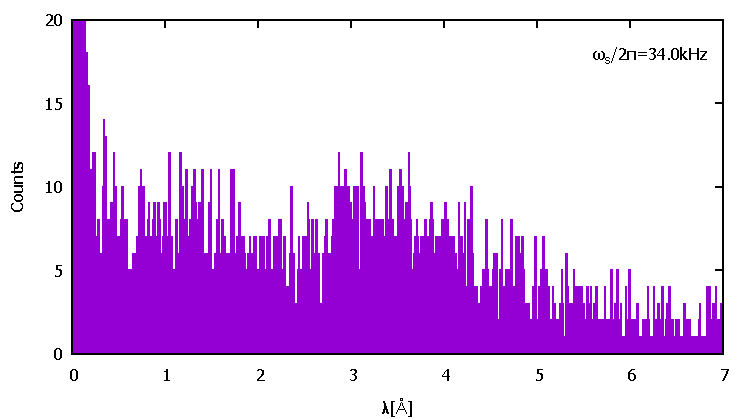
\includegraphics[height=4.3cm]{resonance/results/Flipper1_RawCounts_340kHz.pdf}
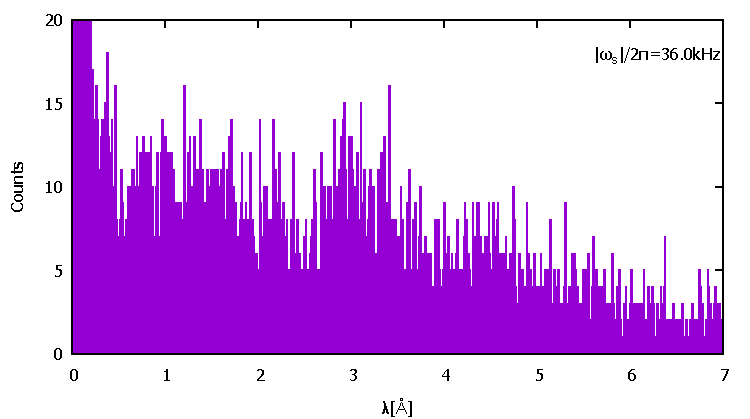
\includegraphics[height=4.3cm]{resonance/results/Flipper1_RawCounts_360kHz.pdf}\\
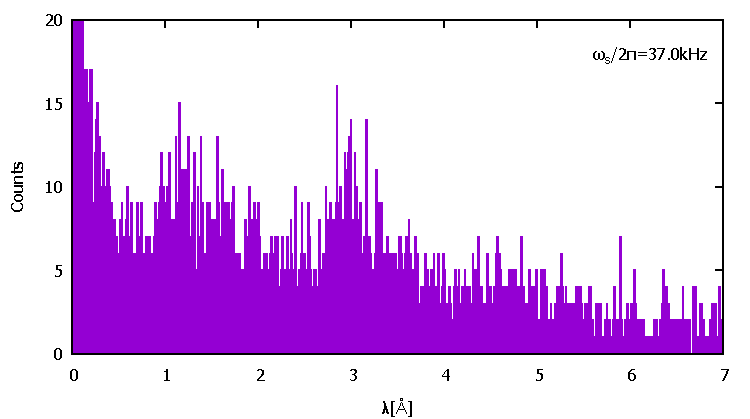
\includegraphics[height=4.3cm]{resonance/results/Flipper1_RawCounts_370kHz.pdf}
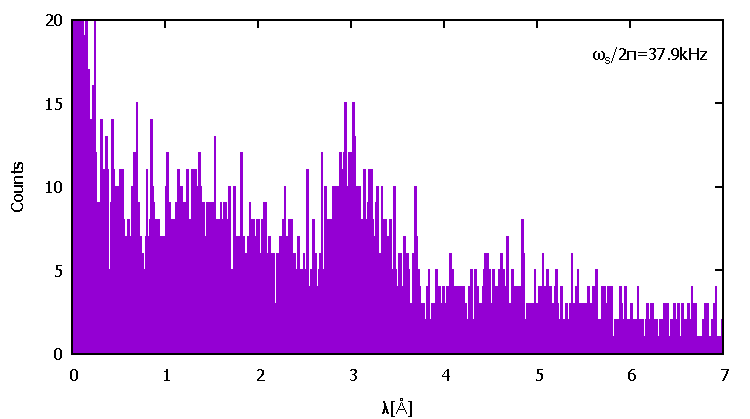
\includegraphics[height=4.3cm]{resonance/results/Flipper1_RawCounts_379kHz.pdf}\\
%\end{minipage}
%\begin{minipage}{0.49\hsize}
%\centering
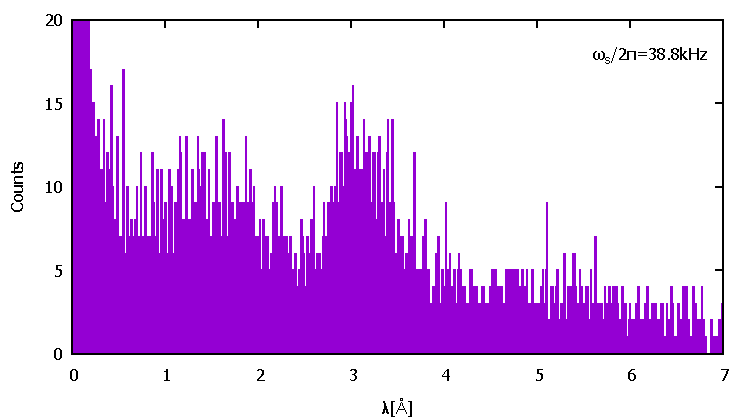
\includegraphics[height=4.3cm]{resonance/results/Flipper1_RawCounts_388kHz.pdf}
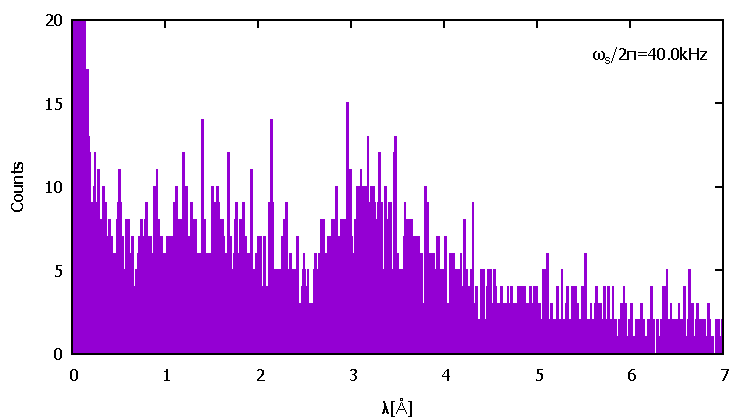
\includegraphics[height=4.3cm]{resonance/results/Flipper1_RawCounts_400kHz.pdf}\\
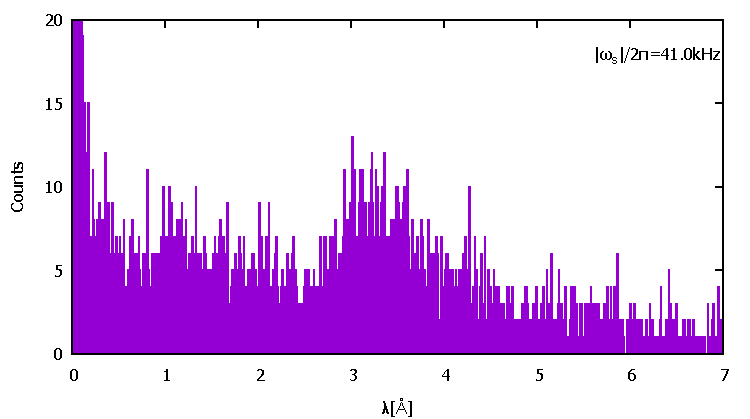
\includegraphics[height=4.3cm]{resonance/results/Flipper1_RawCounts_410kHz.pdf}
%\vspace{4.3cm}
%\end{minipage}
\caption{上流フリッパー共鳴実験で得られた粒子数の波長分布}\label{Resonance_fig_Flipper1_RawCounts}
\end{figure}

\begin{figure}[h]
%\begin{minipage}{0.5\hsize}
%\centering
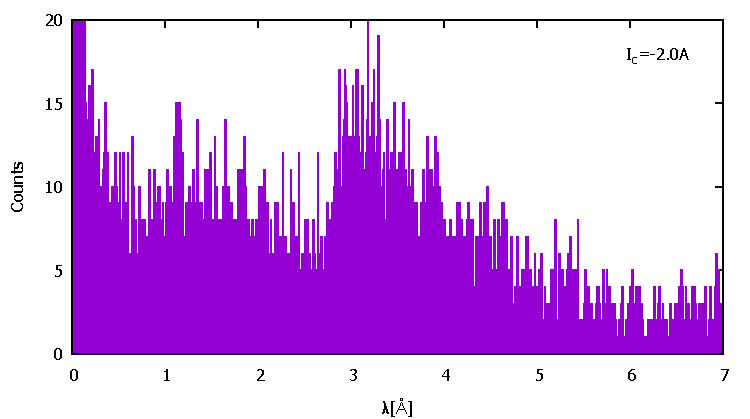
\includegraphics[height=4.3cm]{resonance/results/Flipper2_RawCounts_-20A.pdf}
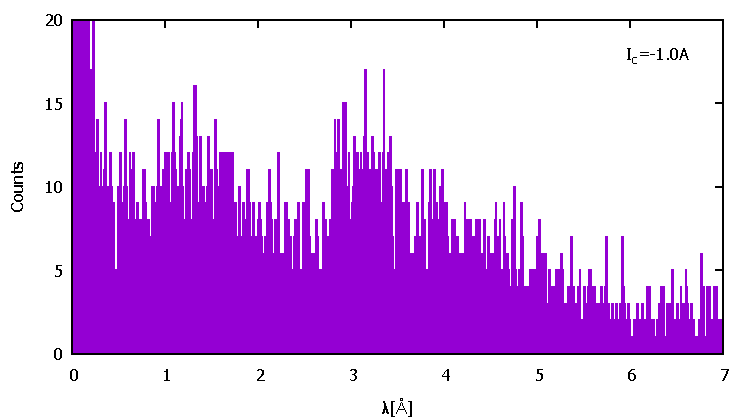
\includegraphics[height=4.3cm]{resonance/results/Flipper2_RawCounts_-10A.pdf}\\
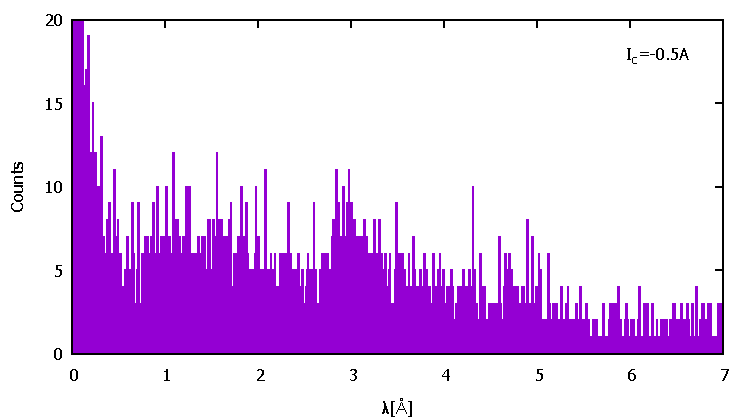
\includegraphics[height=4.3cm]{resonance/results/Flipper2_RawCounts_-5A.pdf}
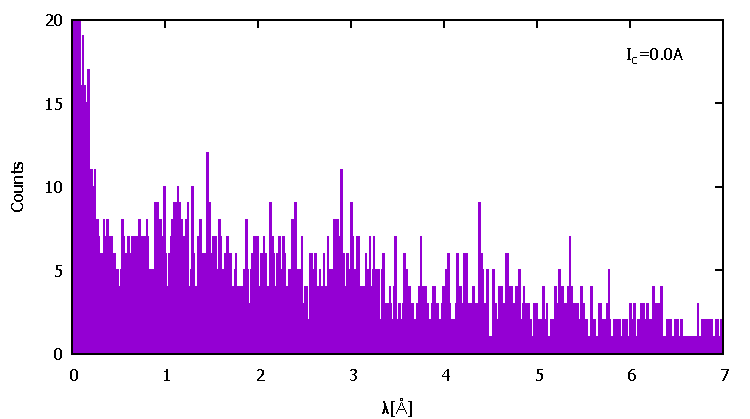
\includegraphics[height=4.3cm]{resonance/results/Flipper2_RawCounts_0A.pdf}\\
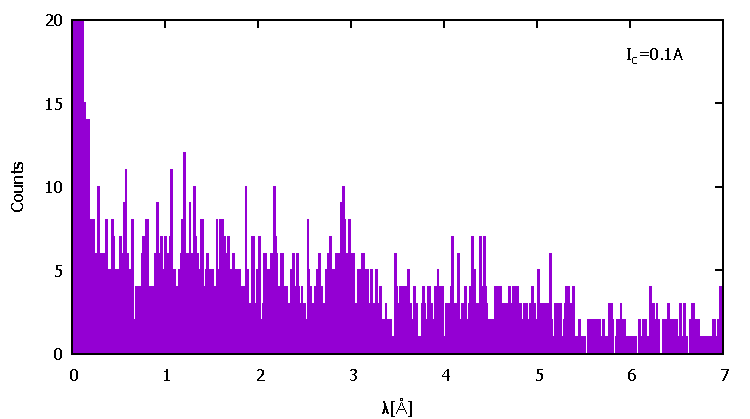
\includegraphics[height=4.3cm]{resonance/results/Flipper2_RawCounts_1A.pdf}
%\end{minipage}
%\begin{minipage}{0.5\hsize}
%\centering
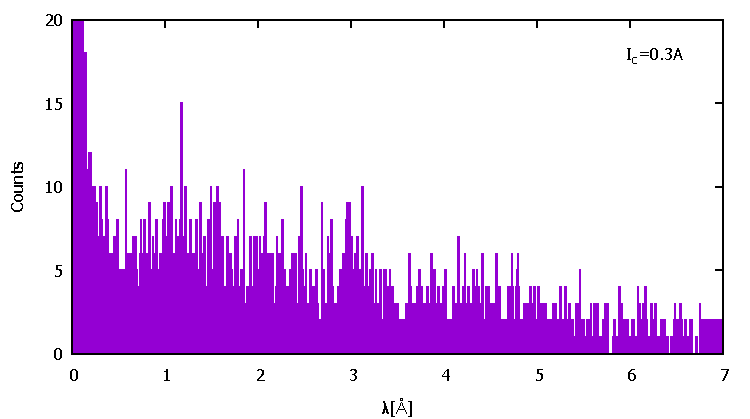
\includegraphics[height=4.3cm]{resonance/results/Flipper2_RawCounts_3A.pdf}\\
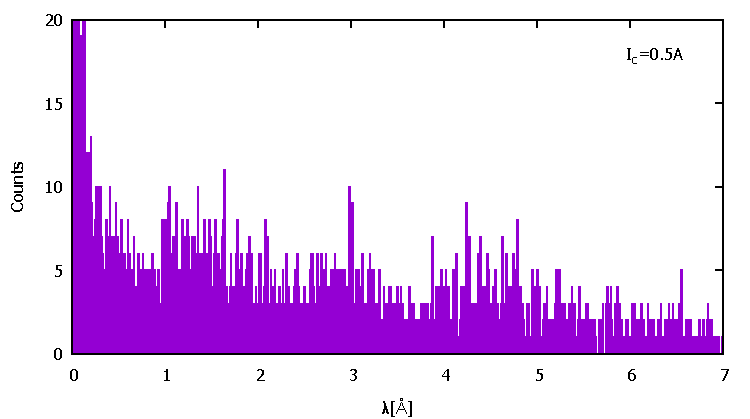
\includegraphics[height=4.3cm]{resonance/results/Flipper2_RawCounts_5A.pdf}
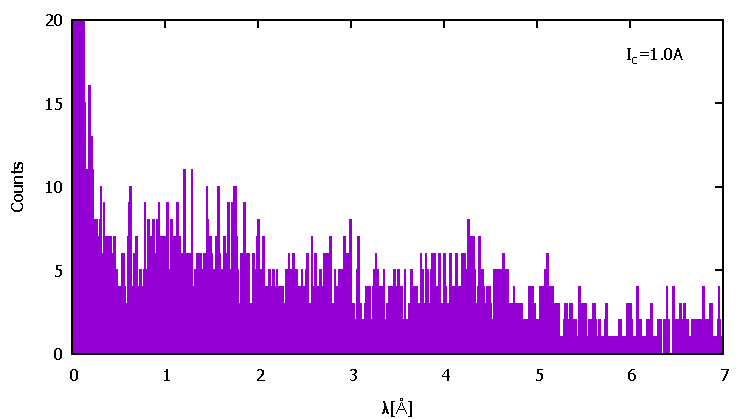
\includegraphics[height=4.3cm]{resonance/results/Flipper2_RawCounts_10A.pdf}\\
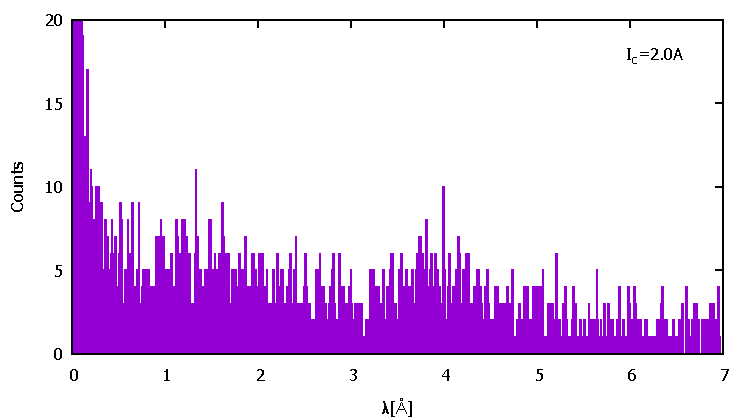
\includegraphics[height=4.3cm]{resonance/results/Flipper2_RawCounts_20A.pdf}
%\vspace{4.3cm}
%\end{minipage}
\caption{下流フリッパー共鳴実験で得られた粒子数の波長分布}\label{Resonance_fig_Flipper2_RawCounts}
\end{figure}

\clearpage
\subsection{分析}
以下では
\begin{enumerate}
\item 上流フリッパーについてデータから共鳴条件を満たす$\omega_s$を決め、グラフから共鳴時に最もよくスピン反転する中性子の波長を推定し、$\pi$フリップ条件から$\omega_r$を計算する。
\item 上流フリッパーについてデータから共鳴条件を満たす$I_c$を決め、グラフから共鳴時に最もよくスピン反転する中性子の波長を推定し、$\pi$フリップ条件から$\omega_r$を計算する。
\end{enumerate}
という流れでデータの分析を行う。

\paragraph{上流フリッパーに関する分析}
共鳴しているかを知るにはパラメータを変えたときの検出粒子数を比較すればよく、ある波長でカウントが最小となるとき共鳴していると考えてよい。しかし前節で示したデータは測定時間や加速器の出力がそれぞれ異なるので、そのままでは互いに比較することができない。そこで測定データのカウントをそのデータの測定開始時刻から測定終了時刻までにおけるLiMのカウントで割って規格化することで、データを互いに比較できるようにする。このようにして規格化した上流フリッパー共鳴実験における粒子数の波長分布を、フリッパーをOFFにしたときの規格化粒子数と共に、図\ref{Resonance_fig_Flipper1_NormalizedCounts}に表す。

\begin{figure}[h]
%\begin{minipage}{0.49\hsize}
%\centering
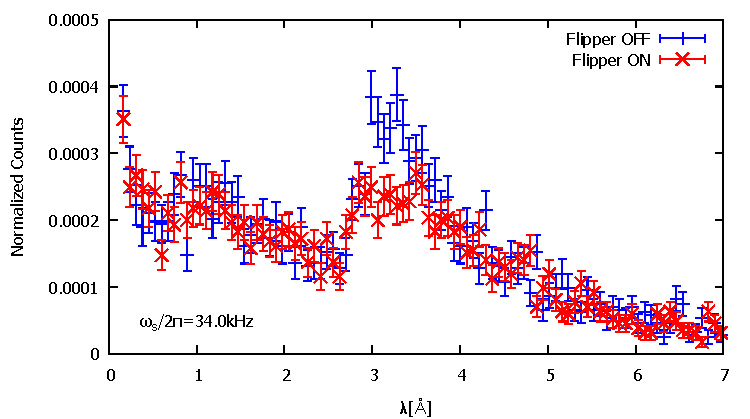
\includegraphics[height=4.3cm]{resonance/analysis/Flipper1_NormalizedCounts_340kHz.pdf}
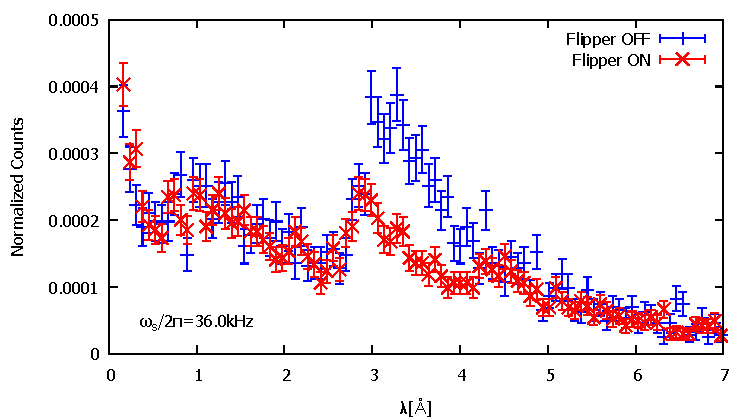
\includegraphics[height=4.3cm]{resonance/analysis/Flipper1_NormalizedCounts_360kHz.pdf}\\
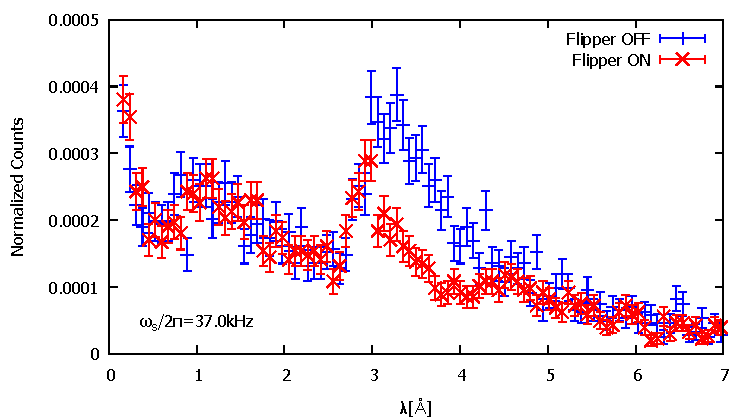
\includegraphics[height=4.3cm]{resonance/analysis/Flipper1_NormalizedCounts_370kHz.pdf}
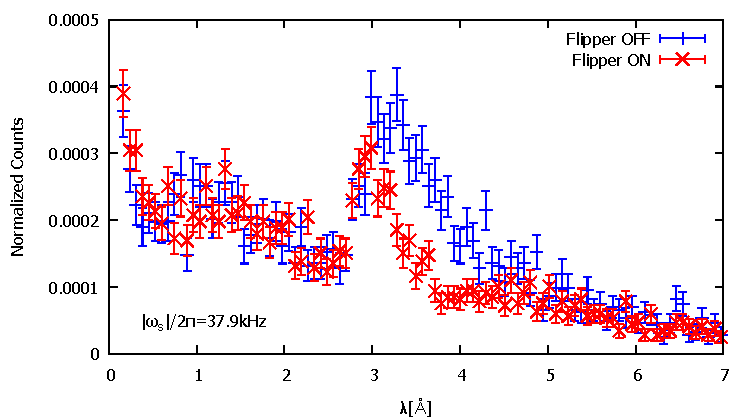
\includegraphics[height=4.3cm]{resonance/analysis/Flipper1_NormalizedCounts_379kHz.pdf}\\
%\end{minipage}
%\begin{minipage}{0.49\hsize}
%\centering
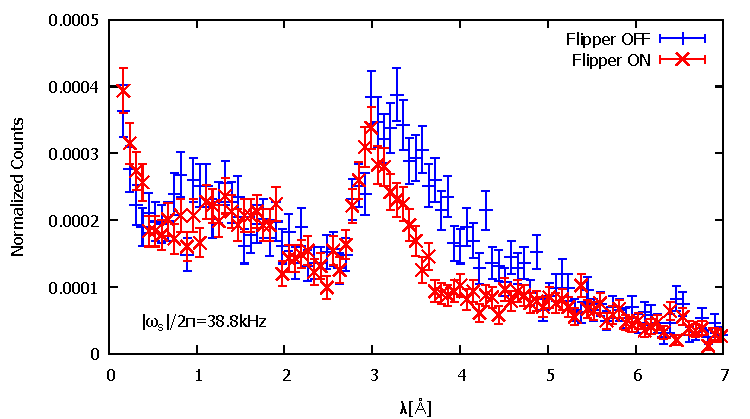
\includegraphics[height=4.3cm]{resonance/analysis/Flipper1_NormalizedCounts_388kHz.pdf}
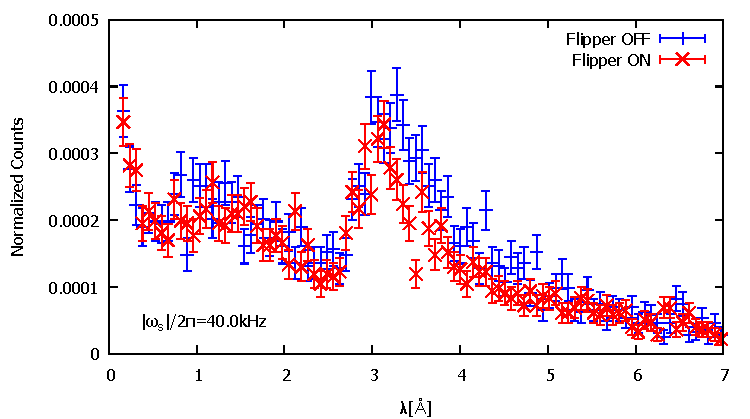
\includegraphics[height=4.3cm]{resonance/analysis/Flipper1_NormalizedCounts_400kHz.pdf}\\
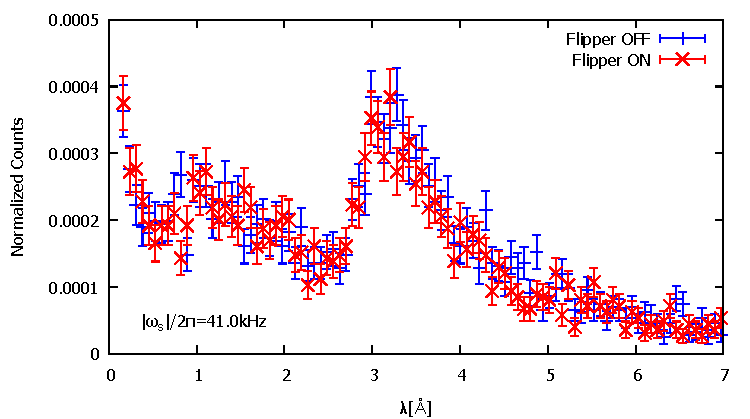
\includegraphics[height=4.3cm]{resonance/analysis/Flipper1_NormalizedCounts_410kHz.pdf}
%\vspace{4.3cm}
%\end{minipage}
\caption{上流フリッパー共鳴実験における規格化粒子数の波長分布}\label{Resonance_fig_Flipper1_NormalizedCounts}
\end{figure}

さらに、図\ref{Resonance_fig_Flipper1_CountsRate}にフリッパーONのときの規格化粒子数をフリッパーOFFのときの規格化粒子数で割ったもの、すなわち上流フリッパーでスピン反転しなかった割合の波長分布を表す。図\ref{Resonance_fig_Flipper1_CountsRate}を見ると、波長$\lambda=$3.0{\AA}から4.5{\AA}あたりで大きく凹んでいることがわかる。
\begin{figure}[h]
%\begin{minipage}{0.49\hsize}
%\centering
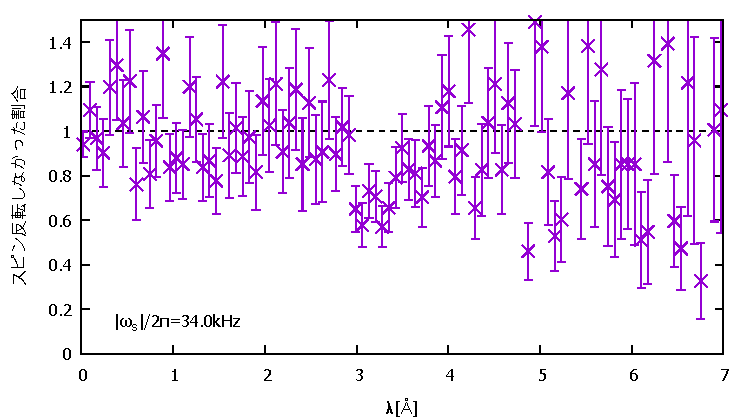
\includegraphics[height=4.3cm]{resonance/analysis/Flipper1_CountsRate_340kHz.pdf}
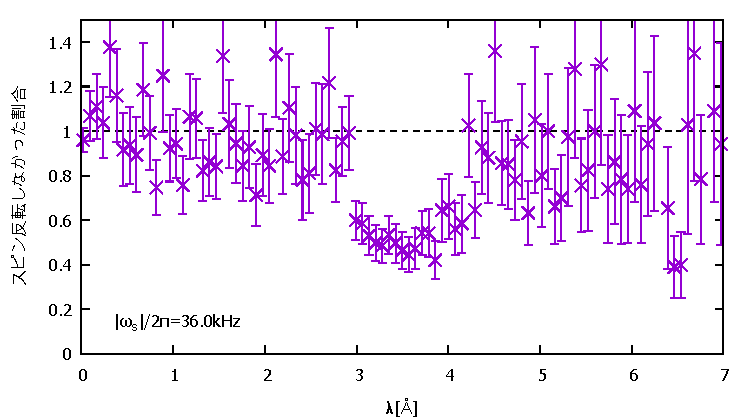
\includegraphics[height=4.3cm]{resonance/analysis/Flipper1_CountsRate_360kHz.pdf}\\
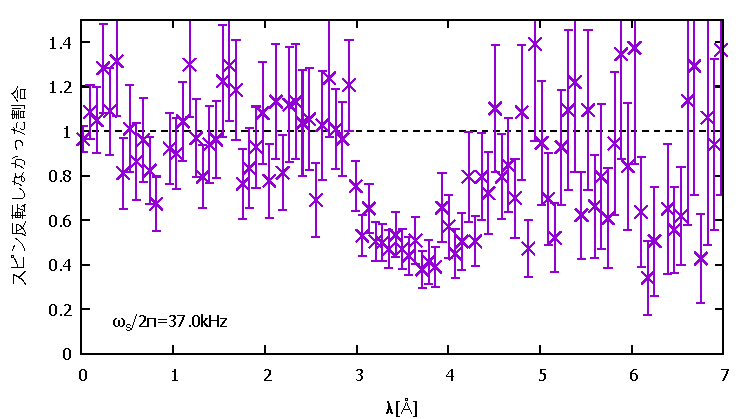
\includegraphics[height=4.3cm]{resonance/analysis/Flipper1_CountsRate_370kHz.pdf}
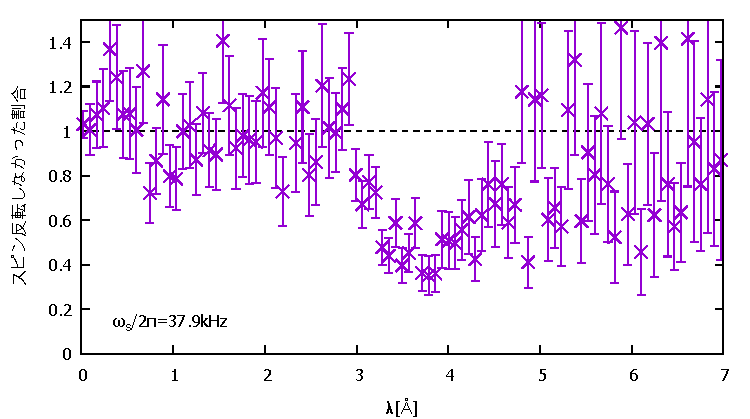
\includegraphics[height=4.3cm]{resonance/analysis/Flipper1_CountsRate_379kHz.pdf}\\
%\end{minipage}
%\begin{minipage}{0.49\hsize}
%\centering
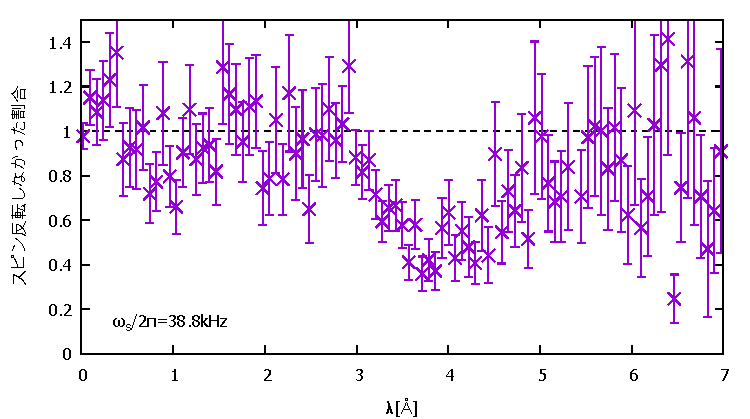
\includegraphics[height=4.3cm]{resonance/analysis/Flipper1_CountsRate_388kHz.pdf}
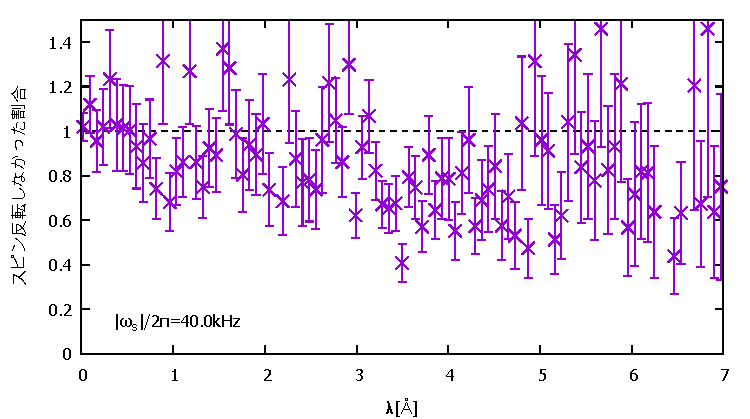
\includegraphics[height=4.3cm]{resonance/analysis/Flipper1_CountsRate_400kHz.pdf}\\
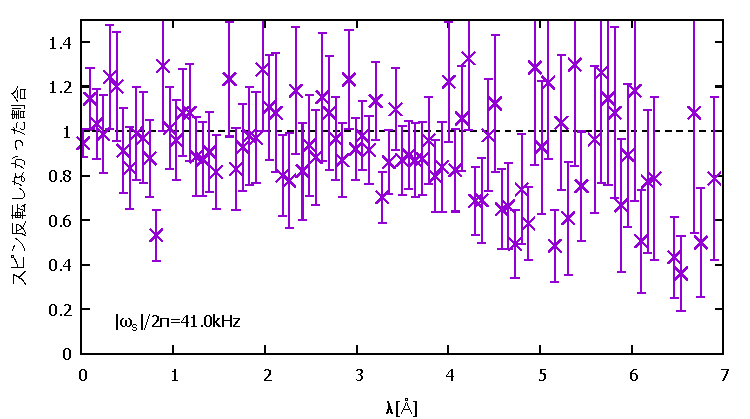
\includegraphics[height=4.3cm]{resonance/analysis/Flipper1_CountsRate_410kHz.pdf}
%\vspace{4.3cm}
%\end{minipage}
\caption{上流フリッパーにおいてスピン反転しなかった割合}\label{Resonance_fig_Flipper1_CountsRate}
\end{figure}

そこで、図\ref{Resonance_fig_Flipper1_NormalizedCounts}の波長領域$\lambda=$3.0{\AA}から4.5{\AA}における規格化粒子数の和を$\omega_s/2\pi$を横軸に取って図示すると図\ref{Resonance_fig_Flipper1_Freq}のようになる。2次関数でフィッティングした結果、最もカウントが少なくなる、すなわち共鳴条件を満たす$\omega_s$として$\omega_s/2\pi=38.0\pm0.1$kHzと決まった。
\begin{comment}
\begin{table}[h]
\centering
\begin{tabular}{c|lllllll}
$\omega_s/2\pi$&34.0&36.0&37.0&37.9&38.8&40.0&41.0\\
$3.0{\AA}-4.5{\AA}での規格化粒子数($\times 10^{-4}$)&$17.8\pm0.8$&18.4\pm
\end{comment}
\begin{figure}[h]
\centering
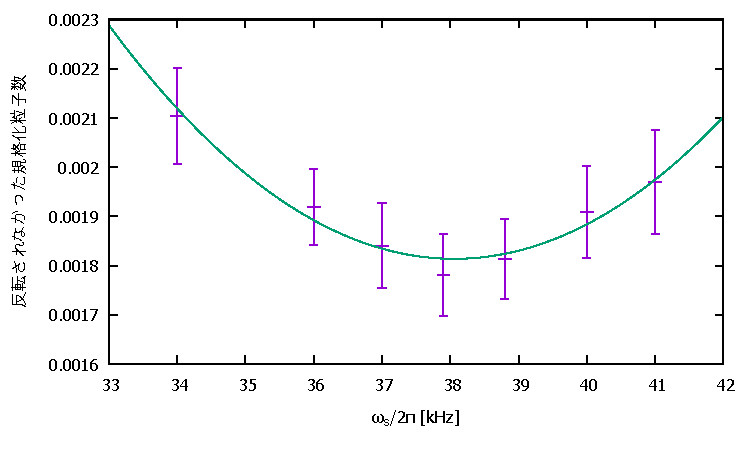
\includegraphics[width=12cm]{resonance/analysis/Flipper1_Freq_30-45.pdf}
\caption{$\omega_s/2\pi$に対する波長$\lambda=$3.0{\AA}から4.5{\AA}における規格化粒子数}\label{Resonance_fig_Flipper1_Freq}
\end{figure}

次に、決まった$\omega_s$と最も近い$\omega_s/2\pi=37.9$kHzのときのスピン反転しなかった割合の波長分布(図\ref{Resonance_fig_Flipper1_CountsRate_379fit})から、最も反転しない割合が低い、すなわち最も反転する波長を推定すると、2次関数フィットの結果、$\lambda=3.78\pm0.05${\AA}と求まった。これを速度に直すと$v=1046\pm14$m/sとなり、この速度が$\pi$フリップ条件を満たすことから$\omega_{r1}/2\pi=8.7\pm0.1$kHzと計算される。
\begin{figure}[h]
\centering
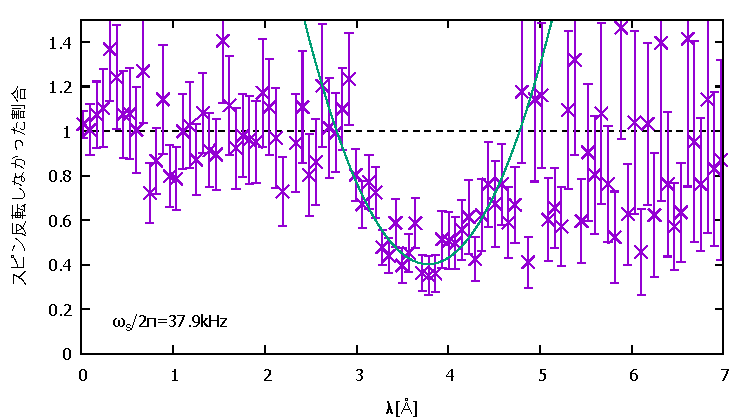
\includegraphics[width=12cm]{resonance/analysis/Flipper1_CountsRate_379kHz_fit.pdf}
\caption{$\omega_s/2\pi$=37.9kHzのときのスピン反転しなかった割合の波長分布}\label{Resonance_fig_Flipper1_CountsRate_379fit}
\end{figure}

\paragraph{下流フリッパーに関する分析}
上流フリッパー同様に下流フリッパーの測定データについても互いに比較するために、測定時間のLiMカウントで規格化を行う。その結果を図\ref{Resonance_fig_Flipper2_NormalizedCounts}に表す。
\begin{figure}[h]
%\begin{minipage}{0.49\hsize}
%\centering
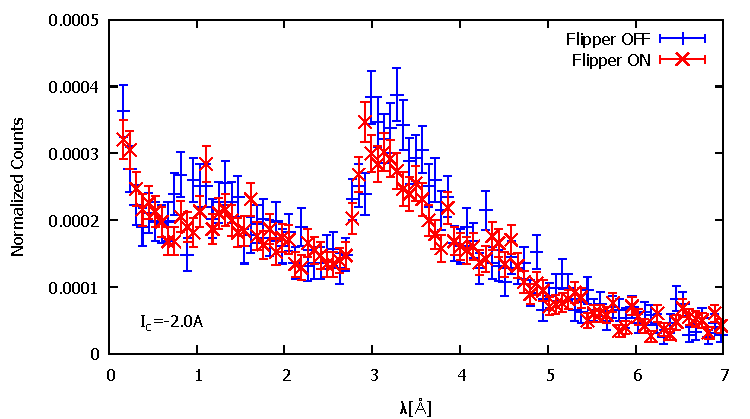
\includegraphics[height=4.3cm]{resonance/analysis/Flipper2_NormalizedCounts_-20A.pdf}
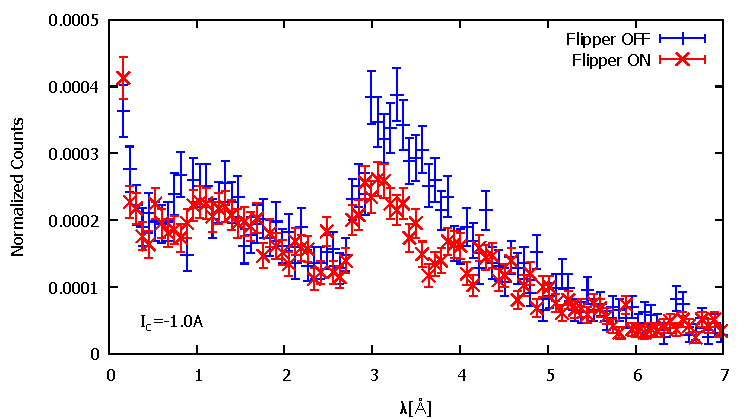
\includegraphics[height=4.3cm]{resonance/analysis/Flipper2_NormalizedCounts_-10A.pdf}\\
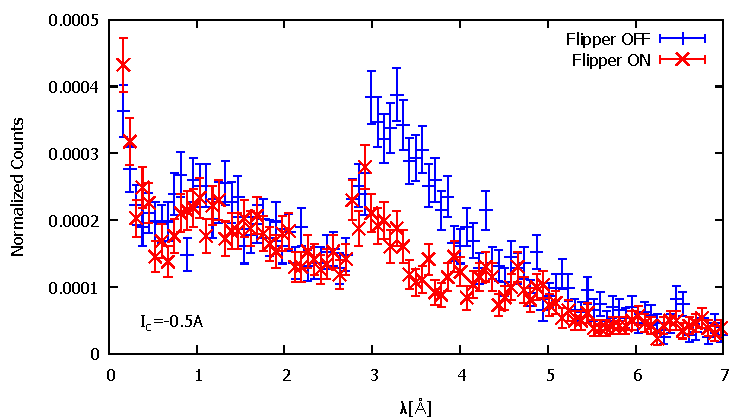
\includegraphics[height=4.3cm]{resonance/analysis/Flipper2_NormalizedCounts_-5A.pdf}
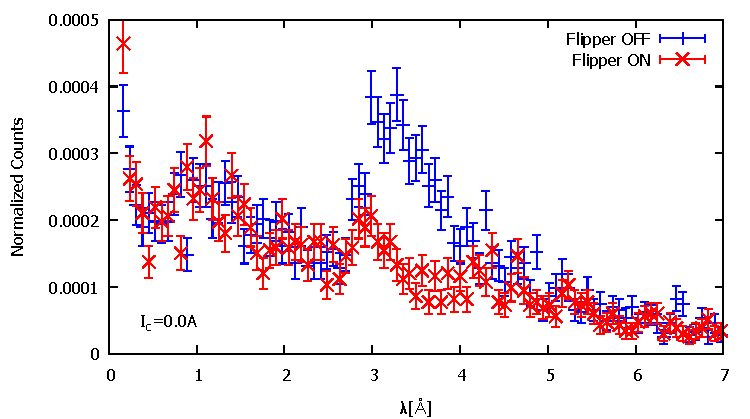
\includegraphics[height=4.3cm]{resonance/analysis/Flipper2_NormalizedCounts_0A.pdf}\\
%\end{minipage}
%\begin{minipage}{0.49\hsize}
%\centering
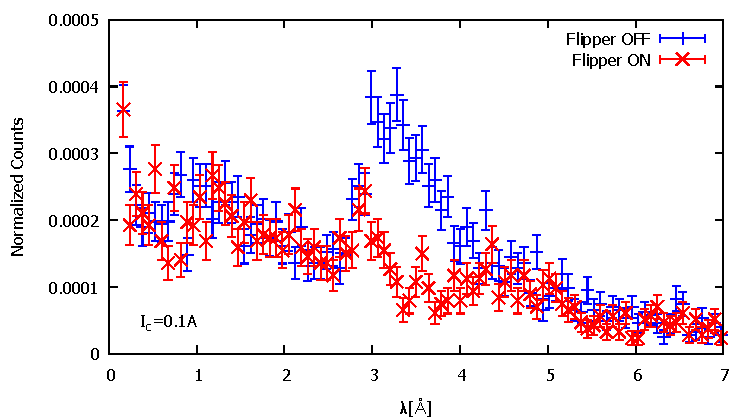
\includegraphics[height=4.3cm]{resonance/analysis/Flipper2_NormalizedCounts_1A.pdf}
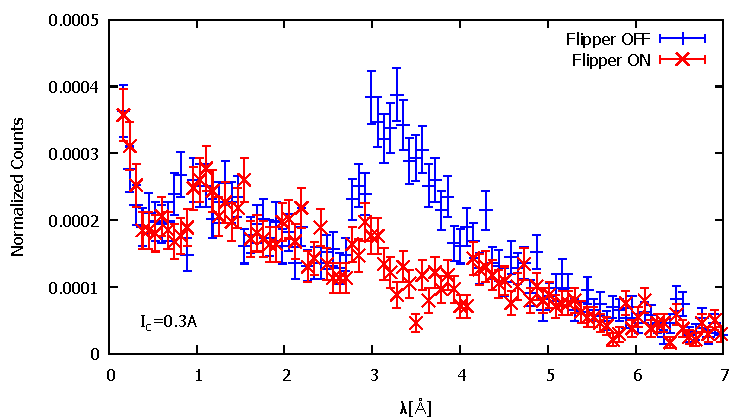
\includegraphics[height=4.3cm]{resonance/analysis/Flipper2_NormalizedCounts_3A.pdf}\\
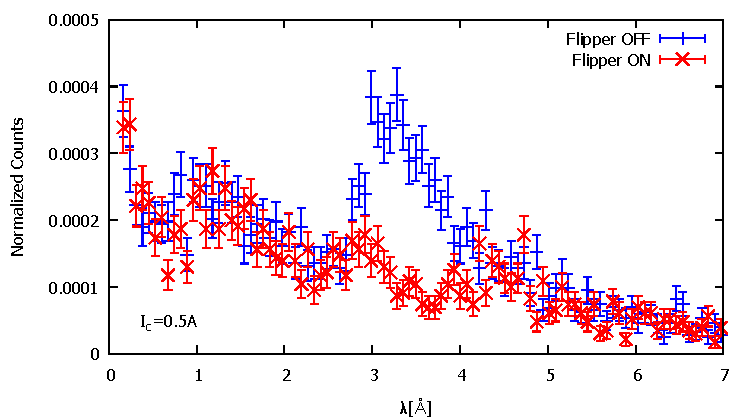
\includegraphics[height=4.3cm]{resonance/analysis/Flipper2_NormalizedCounts_5A.pdf}
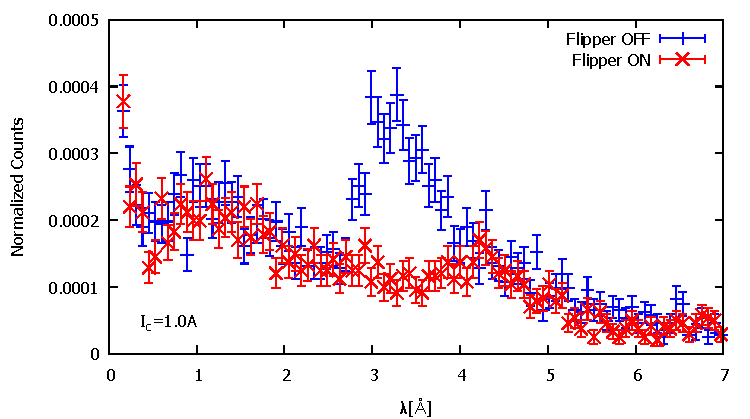
\includegraphics[height=4.3cm]{resonance/analysis/Flipper2_NormalizedCounts_10A.pdf}\\
%\vspace{4.3cm}
%\end{minipage}
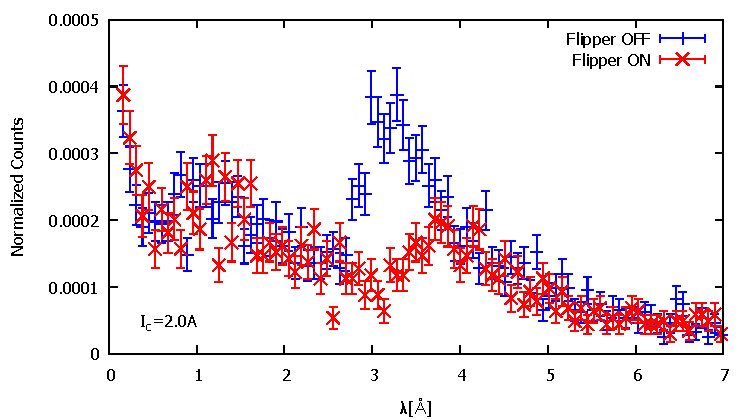
\includegraphics[height=4.3cm]{resonance/analysis/Flipper2_NormalizedCounts_20A.pdf}
\caption{下流フリッパー共鳴実験における規格化粒子数の波長分布}\label{Resonance_fig_Flipper1_NormalizedCounts}
\end{figure}

さらに、図\ref{Resonance_fig_Flipper2_CountsRate}にフリッパーONのときの規格化粒子数をフリッパーOFFのときの規格化粒子数で割ったもの、すなわち上流フリッパーでスピン反転しなかった割合の波長分布を表す。図\ref{Resonance_fig_Flipper2_CountsRate}を見ると、波長$\lambda=$2.7{\AA}から4.2{\AA}あたりで大きく凹んでいることがわかる。
\begin{figure}[h]
%\begin{minipage}{0.49\hsize}
%\centering
\includegraphics[height=4.3cm]{resonance/analysis/Flipper2_CountsRate_-20A.pdf}
\includegraphics[height=4.3cm]{resonance/analysis/Flipper2_CountsRate_-10A.pdf}\\
\includegraphics[height=4.3cm]{resonance/analysis/Flipper2_CountsRate_-5A.pdf}
\includegraphics[height=4.3cm]{resonance/analysis/Flipper2_CountsRate_0A.pdf}\\
%\end{minipage}
%\begin{minipage}{0.49\hsize}
%\centering
\includegraphics[height=4.3cm]{resonance/analysis/Flipper2_CountsRate_1A.pdf}
\includegraphics[height=4.3cm]{resonance/analysis/Flipper2_CountsRate_3A.pdf}\\
\includegraphics[height=4.3cm]{resonance/analysis/Flipper2_CountsRate_5A.pdf}
\includegraphics[height=4.3cm]{resonance/analysis/Flipper2_CountsRate_10A.pdf}\\
%\vspace{4.3cm}
%\end{minipage}
\includegraphics[height=4.3cm]{resonance/analysis/Flipper2_CountsRate_20A.pdf}
\caption{下流フリッパーにおいてスピン反転しなかった割合}\label{Resonance_fig_Flipper2_CountsRate}
\end{figure}

そこで、図\ref{Resonance_fig_Flipper2_NormalizedCounts}の波長領域$\lambda=$2.7{\AA}から4.2{\AA}における規格化粒子数を数え、$I_c$を横軸として図示すると図\ref{Resonance_fig_Flipper2_Cur}のようになる。2次関数でフィッティングした結果、最もカウントが少なくなる、すなわち共鳴条件を満たす$I_c$として$I_c=0.35\pm0.3$Aと決まった。
\begin{figure}[h]
\centering
\includegraphics[width=12cm]{resonance/analysis/Flipper2_Cur_27-42.pdf}
\caption{$I_c$に対する波長$\lambda=$2.7{\AA}から4.2{\AA}における規格化粒子数}\label{Resonance_fig_Flipper2_Cur}
\end{figure}

次に、決まった$I_c$の中心値と最も近い$I_c=0.3$Aのときのスピン反転しなかった割合の波長分布(図\ref{Resonance_fig_Flipper2_CountsRate_3fit})から、最も反転しない割合が低い、すなわち最も反転する波長を推定すると、2次関数フィットの結果、$\lambda=3.48\pm0.05${\AA}と求まった。これを速度に直すと$v=1136\pm16$m/sとなり、この速度が$\pi$フリップ条件を満たすことから$\omega_{r2}/2\pi=9.5\pm0.1$kHzと計算される。
\begin{figure}[h]
\centering
\includegraphics[width=12cm]{resonance/analysis/Flipper2_CountsRate_3A_fit.pdf}
\caption{$I_c$=0.3Aのときのスピン反転しなかった割合の波長分布}\label{Resonance_fig_Flipper2_CountsRate_3fit}
\end{figure}

\clearpage
\paragraph{分析まとめ}
以上の分析から各パラメータは次のように決まった。
\begin{table}[h]
\centering
\begin{tabular}{|c|c|} \hline
$\omega_s/2\pi$&$38.0\pm0.1$kHz\\ \hline
$I_c$&$0.35\pm0.3$A \\ \hline
$\omega_{r1}/2\pi$&$8.7\pm0.1$kHz \\ \hline
$\omega_{r2}/2\pi$&$9.5\pm0.1$kHz \\ \hline
\end{tabular}
\end{table}

しかし、実験中の粗い解析では$\omega_s/2\pi=37.5\pm0.1$kHz,$I_c=0.185\pm0.11$Aと求まったため、実際には以後、
\begin{table}[h]
\centering
\begin{tabular}{|c|c|} \hline
$\omega_s/2\pi$&37.5kHz\\ \hline
$I_c$&0.185A \\ \hline
\end{tabular}
\end{table}

\noindent として実験を進めた。このことによる共鳴条件からのずれは共に$\epsilon/\omega_z=$0.01$\sim$0.02程度であり、十分小さいといえる(図\ref{Resonance_fig_visivility},\ref{Resonance_fig_interference}参照)。
